%%%%%%%%%%%%%%%%%%%%%%%%%%
% A template for Master's Thesis
% Systems Security Group
% Coventry University
% 2025
%%%%%%%%%%%%%%%%%%%%%%%%%%


\documentclass[12pt,oneside]{book}

%% ======================================================================
%% Document geometry and layout
%% ======================================================================
\usepackage[margin=1.2in]{geometry}  % Page margins
\usepackage{fancyhdr}                % Custom headers and footers
\usepackage{setspace}                % Line spacing control
\usepackage{microtype}               % Typography improvements (character protrusion, font expansion)

%% ======================================================================
%% Document structure packages
%% ======================================================================
\usepackage[toc,page]{appendix}      % Improved appendix handling
\usepackage{pdfpages}                % Include PDF documents
\usepackage{enumitem}                % Customizable lists
\usepackage{lipsum}                  % Dummy text generator

%% ======================================================================
%% Graphics and color packages
%% ======================================================================
\usepackage{graphicx}                % Enhanced graphics support
\graphicspath{{./images/}{./figures/}}
\usepackage{xcolor}                  % Extended color support
\usepackage{float}                   % Improved figure positioning
% \usepackage{subfig}                  % Subfigures within figures
\usepackage{placeins}                % Control float placement
\usepackage{wrapfig}                % Wrap text around figures
\usepackage{lscape}                  % Landscape orientation for pages

%% ======================================================================
%% Mathematical typesetting
%% ======================================================================
\usepackage{amsmath, amssymb, amsfonts, amsthm}  % AMS mathematics packages
\usepackage{siunitx}                 % SI units formatting
\usepackage{tikz}                    % Drawing diagrams
\usepackage{pgfplots}                % Plotting functions and data
\usepackage{tikz-cd}                 % Commutative diagrams
\usetikzlibrary{arrows,shapes,positioning,calc,patterns,decorations.pathmorphing,decorations.markings}
\pgfplotsset{compat=newest}

%% ======================================================================
%% Table packages
%% ======================================================================
\usepackage{booktabs}                % Professional tables
\usepackage{longtable}               % Tables spanning multiple pages
\usepackage{multirow}                % Multiple row cells
\usepackage{tabularx}                % Flexible table columns

%% ======================================================================
%% Bibliography and references
%% ======================================================================
\usepackage{natbib}  % Bibliography style

%% ======================================================================
%% Algorithms and code listings
%% ======================================================================
\usepackage{algorithm2e}             % Algorithms
\usepackage{listings}                % Code listings
\lstset{
  basicstyle=\ttfamily\small,
  breaklines=true,
  commentstyle=\color{green!60!black},
  keywordstyle=\color{blue},
  stringstyle=\color{red},
  numbers=left,
  numberstyle=\tiny\color{gray},
  numbersep=5pt
}

%% ======================================================================
%% Hyperlinks - load this last to avoid conflicts
%% ======================================================================
\usepackage[colorlinks=true, 
            linkcolor=blue, 
            citecolor=blue, 
            urlcolor=blue,
            bookmarks=true,
            bookmarksopen=true]{hyperref}

%% ======================================================================
%% Captions and references
%% ======================================================================
\usepackage{caption}
\usepackage{subcaption}
\usepackage{cleveref}                % Intelligent cross-referencing


\begin{document}

\captionsetup[figure]{margin=1.5cm,font=small,labelfont={bf},name={Figure},labelsep=colon,textfont={it}}
\captionsetup[table]{margin=1.5cm,font=small,labelfont={bf},name={Table},labelsep=colon,textfont={it}}
\SetLipsumDefault{1}

\frontmatter

\begin{titlepage}


% -------------------------------------------------------------------
% You need to edit the details here
% -------------------------------------------------------------------

\begin{center}
{\LARGE Coventry University}\\[0.25cm]
{\Large Faculty of Engineering, Environment and Computing
School of Computing, Electronics and Mathematics 
}\\[1.5cm]
\linespread{1.2}\huge {\bfseries Leveraging Machine Learning for Network Malware Detection}\\[1cm]
\linespread{1}
\includegraphics[width=6.5cm]{culogo.JPG}\\[1.5cm]
{\Large\bf Ekwunife Blessing Ifunanya  }\\[0.25cm]
{\large \emph{Student ID:} 15116185}\\[0.25cm]
{\large \emph{Supervisor:} Dr. Kabiru Mohammed}\\[1cm] % if applicable
\vspace{\fill}
\large Submitted in partial fulfillment of the University's requirements\\ for the degree of Master of Science in cybersecurity\\[0.5cm]
\large Academic Year: 2024/25
\end{center}

\end{titlepage}


% -------------------------------------------------------------------
% Declaration
% -------------------------------------------------------------------

\newpage
\section*{Declaration of Originality}

I declare that this project is all my own work and has not been copied in part or in whole from any other source except where duly acknowledged. As such, all use of previously published work (from books, journals, magazines, internet etc.) has been acknowledged by citation within the main report to an item in the References or Bibliography lists. I also agree that an electronic copy of this project may be stored and used for the purposes of plagiarism prevention and detection.

\bigskip

\section*{Statement of copyright}
I acknowledge that the copyright of this project report, and any product developed as part of the project, belong to Coventry University. Support, including funding, is available to commercialise products and services developed by staff and students. Any revenue that is generated is split with the inventor/s of the product or service. For further information please see \href{https://www.coventry.ac.uk/ipr}{www.coventry.ac.uk/ipr} or contact 
\href{mailto:ipr@coventry.ac.uk}{ipr@coventry.ac.uk}.

\bigskip

\section*{Statement of ethical engagement}
I declare that a proposal for this project has been submitted to the Coventry University ethics monitoring website (\href{https://ethics.coventry.ac.uk/}{https://ethics.coventry.ac.uk/}) and that the application number is listed below (Note: Projects without an ethical application number will be rejected for marking)

\bigskip
% \includegraphics[width=1.5cm]{output.png}
\noindent Name: Ekwunife Blessing Ifunanya\\[1mm]
\rule[1em]{25em}{0.5pt}

\noindent Signature: EBI\\[1mm]
\rule[1em]{25em}{0.5pt}

\noindent Date: 13/04/2025\\[1mm]
\rule[1em]{25em}{0.5pt}

\noindent Student ID: 15116185\\[1mm]
\rule[1em]{25em}{0.5pt}

\noindent Ethics Application Number: P184895\\[1mm]
\rule[1em]{25em}{0.5pt}

\noindent 1st Supervisor Name: Dr. Kabiru Mohammed\\[1mm]
\rule[1em]{25em}{0.5pt}

\noindent 2nd Supervisor Name: Dr. Antal Goldschmidt\\[1mm]
\rule[1em]{25em}{0.5pt}

% \includepdf[pages=-]{forms/form.pdf}

\chapter*{\Large \center Acknowledgement}

\noindent I will like to express my sincere gratitude to my supervisor, Dr. Kabiru Mohammed, for his invaluable guidance and support throughout this research project. His expertise and insights have been instrumental in shaping the direction of my work and ensuring its success. I would also like to thank my parents for their unwavering support and encouragement throughout my academic journey. Their belief in my abilities has motivated me to strive for excellence in all of my endeavours. Finally, I would like to acknowledge the contributions of my peers and colleagues at Coventry University, whose collaboration and camaraderie have made this experience enjoyable and enriching. Thank you for your support.

\newpage

% -------------------------------------------------------------------
% Abstract
% -------------------------------------------------------------------

\chapter*{\Large \center Abstract}

This research investigates the application of machine learning techniques for detecting malware in Internet of Things (IoT) network traffic. As IoT devices proliferate across homes and critical infrastructure, they present attractive targets for cyber attacks due to their inherent security limitations. This study leverages the CTU-IoT-Malware dataset, which contains approximately one million labelled network connections, to develop and evaluate models capable of distinguishing between benign and malicious traffic patterns.

The research implements a comprehensive methodology that involves extensive data pre-processing, feature engineering, and the development of multiple machine learning models. Exploratory data analysis revealed distinct patterns in protocol usage, connection states, and temporal behaviour between benign and malicious traffic. TCP dominated malicious traffic (72.4\% vs 40.9\% in benign), with the state of connection S0 (connection attempt without reply) representing 94. 7\% of malicious connections, strongly indicative of scanning behaviour.

Four classification approaches were implemented and compared: Random Forest, Support Vector Machine (SVM), XGBoost, and a custom neural network architecture. The models were rigorously evaluated using metrics including accuracy, precision, recall, F1 score, and area under the ROC curve. The optimised Random Forest model achieved the highest overall performance with 99.8\% accuracy and 0.998 F1 score, slightly outperforming the neural network (99.6\% accuracy). Feature importance analysis revealed that connection state, protocol type, and metrics derived such as bytes per packet ratios were particularly influential in classification decisions. The research contributes valuable information for the development of lightweight and effective IoT security monitoring solutions by identifying the most discriminative features of network traffic and quantifying the effectiveness of various machine learning approaches for malware detection in resource-constrained environments.

\vspace{0.5cm}
\textbf{Keywords:} IoT Security, Network Traffic Analysis, Machine Learning, Malware Detection, Random Forest, Deep Learning


% -------------------------------------------------------------------
% Contents, list of figures, list of tables
% -------------------------------------------------------------------

\tableofcontents
\listoffigures
\listoftables


% -------------------------------------------------------------------
% Main sections (as required)
% -------------------------------------------------------------------

\mainmatter

\chapter{Introduction}

\section{Background and Motivation}

The rapid proliferation of devices on the Internet of Things (IoT) has fundamentally transformed modern network infrastructures, creating unprecedented security challenges for organisations and individuals alike. With the projected number of connected IoT devices exceeding 30 billion by 2025 \citep{Cisco2020}, and the global market value approaching £1.2 trillion by 2027 \citep{IoTAnalytics2021}, these technologies have become integral to critical infrastructure, industrial systems, healthcare and consumer applications. Although IoT technologies deliver significant benefits in automation, efficiency, and data-driven decision making, they simultaneously introduce substantial cybersecurity vulnerabilities that traditional protection mechanisms struggle to address.

IoT environments present unique security concerns that differentiate them from conventional information technology infrastructures. These challenges arise from several interconnected factors: the heterogeneous nature of IoT ecosystems, comprising devices with vastly different hardware capabilities, operating systems, and communication protocols; the widespread deployment of resource-constrained devices with limited processing power, memory, and energy capacity; minimal built-in security controls due to cost considerations and manufacturing priorities; and an exponentially expanded attack surface created by the large number of network-connected devices \citep{Bertino2017, Neshenko2019}.

The threat landscape targeting IoT ecosystems has evolved with alarming sophistication. The Mirai botnet attack in 2016 demonstrated the devastating potential of malware aimed at the Internet of Things, compromising more than 600,000 vulnerable devices to launch unprecedented distributed denial of service attacks against critical internet infrastructure \citep{Antonakakis2017}. This watershed event fundamentally altered perceptions of IoT security, revealing systemic vulnerabilities that continue to be exploited. More recent threats such as Mozi, Dark Nexus, and Torii have significantly expanded the arsenal of IoT-specific malware, targeting an ever-wider range of devices and leveraging increasingly advanced persistence and propagation mechanisms \citep{Kambourakis2021, Mehrban2021}.

Conventional security approaches based on signature-based detection, static rule sets, and perimeter defences have been found to be woefully inadequate to protect IoT environments \citep{Nguyen2019}. These methods rely on identifying known attack patterns rather than detecting novel threats and struggle to adapt to the polymorphic nature of modern malware. Furthermore, the resource limitations of many IoT devices preclude the deployment of conventional endpoint protection solutions, such as antivirus software or host-based intrusion detection systems. This reality requires the development of network-based monitoring approaches capable of identifying malicious activity without imposing a computational burden on the devices themselves \citep{Diro2018}.

Machine learning presents a promising paradigm for addressing these challenges, offering the potential for more adaptive and scalable detection capabilities that can operate effectively in dynamic IoT environments \citep{Buczak2016}. By recognising patterns in network traffic that indicate malicious activity, machine learning models can identify both known threats and potential zero-day attacks that evade signature-based systems. Recent research has demonstrated encouraging results using various algorithms including Random Forest, Support Vector Machines, and deep learning approaches for network intrusion detection in IoT contexts \citep{Aldweesh2020, Diro2021}.

However, developing effective machine learning solutions for IoT security monitoring introduces distinct challenges. These include identifying the optimal set of network traffic features that balance discriminative power with computational efficiency; selecting appropriate algorithms that can operate effectively within the resource constraints of IoT environments; achieving acceptable detection accuracy while minimising false positives that could overwhelm security analysts; and ensuring model interpretability to enable meaningful response to detected threats \citep{Vinayakumar2019, baich2022machine, saran2023comparative}.

In this research, I investigate the application of machine learning for network-based malware detection in IoT environments, with a particular focus on developing practical approaches that balance detection efficacy with operational viability. By analysing network traffic data from the CTU-IoT-Malware dataset, I aim to identify efficient feature sets and develop optimised models capable of distinguishing between benign and malicious communications across diverse attack vectors, whilst remaining suitable for deployment in resource-constrained monitoring environments.

\section{Aims and Objectives}

The primary aim of this research is to develop effective machine learning approaches for detecting malware in IoT network traffic that balance detection accuracy with computational efficiency for practical deployment in resource-constrained IoT environments.

To achieve this aim, I have established the following specific objectives.

\begin{enumerate}
    \item Identify the features of network traffic that most effectively distinguish between benign and malicious communications in IoT environments through a comprehensive exploratory analysis.
    
    \item Develop and implement optimised feature selection methodologies that identify the minimal set of discriminative traffic attributes whilst minimising computational complexity.
    
    \item To design and evaluate machine learning models for classification and determine which machine learning algorithms (including Random Forest, Support Vector Machines, XGBoost, and deep learning approaches) provide the optimal balance between detection accuracy, false positive rates, and computational efficiency.
    
    \item Optimise the model parameters and architectures to enhance detection performance, ensuring their applicability in IoT monitoring environments. Evaluate the impact of various preprocessing, feature engineering, and dimensionality reduction methods on model performance. Assess model interpretability using feature importance and explainable AI techniques, offering actionable insights for security professionals.
    
\end{enumerate}

Through achieving these objectives, my aim is to contribute practical security monitoring solutions that can enhance the protection of IoT systems against increasingly sophisticated threats while operating within the unique constraints of these environments.

\section{Significance of the Research}

This research addresses significant challenges in the cybersecurity domain, particularly in relation to IoT environments. The contributions of this work include the following:

\begin{itemize}
    \item By identifying the most effective features and models for network-based malware detection in IoT contexts, I provide practical guidance to security teams that implement monitoring solutions in resource-constrained environments.
    
    \item  Through systematic comparison and optimisation of different machine learning approaches, my work contributes to the growing body of knowledge on AI-driven security solutions tailored to IoT environments.
    
    \item The comprehensive exploratory analysis of the traffic characteristics of the IoT network offers valuable insights into both normal behaviour and attack patterns specific to these environments, improving our understanding of the threat landscapes of the IoT.
    
    \item By identifying the minimal set of traffic features needed for effective detection, I support the development of more efficient monitoring solutions suitable for deployment in environments with limited computational resources.
    
    \item By emphasising the importance of model interpretability alongside performance metrics, my research addresses a critical need for explainable AI in security contexts where understanding model decisions is essential for incident response.
\end{itemize}

As IoT adoption continues to accelerate across industries, the need for effective security monitoring becomes increasingly urgent. My research addresses this need through a systematic investigation of machine learning approaches that can enhance the protection of these critical systems while operating within their unique constraints.
\chapter{Literature Review}

\section{Introduction}

The security challenges posed by the Internet of Things (IoT) devices have attracted significant research attention in recent years. This chapter presents a critical examination of the existing literature relevant to malware detection in IoT networks using machine learning techniques. The review is structured around five key areas: (1) security challenges specific to IoT environments, (2) network-based approaches to malware detection, (3) machine learning techniques for network traffic analysis, (4) feature selection and dimensionality reduction in network security applications, and (5) evaluation frameworks and datasets for IoT security research. Throughout this review, I identify the current state of knowledge, highlight existing research gaps, and position my research within the broader academic discourse.

\section{Security Challenges in IoT Environments}

IoT ecosystems present unique security challenges that differentiate them from conventional IT infrastructures. These challenges arise from the inherent characteristics of IoT deployments and have been thoroughly documented in the literature.

\subsection{Resource Constraints and Security Implications}

The resource-constrained nature of many IoT devices fundamentally limits their security capabilities. \cite{Bertino2017} conducted a comprehensive analysis of IoT security challenges, highlighting that limited computational power, memory, and energy capacity prevent the implementation of robust security mechanisms directly on devices. Their work demonstrated that lightweight cryptographic protocols often provide insufficient protection against sophisticated attacks, while more robust security implementations may exceed device capabilities or severely impact operational performance.

Building on this foundation, \cite{Neshenko2019} provided an exhaustive survey of IoT vulnerabilities, identifying three main categories of constraints that affect security: hardware limitations, software limitations, and networking constraints. Their analysis of more than 300 documented IoT exploits revealed that 68\% leveraged vulnerabilities directly attributable to device resource constraints. The authors concluded that these constraints require novel security approaches that can operate effectively without imposing a significant burden on the devices themselves.

\subsection{Heterogeneity and Standardisation Challenges}

The heterogeneous nature of IoT deployments creates significant security management challenges. Securing IoT deployments is a multifaceted challenge that requires a comprehensive approach to address the unique vulnerabilities and threats associated with IoT systems. The distributed nature of IoT, combined with the diversity of devices and communication protocols, requires robust security measures to protect data integrity, confidentiality, and availability. \cite{bhattacharjee2018practical} examined the security implications of device heterogeneity in industrial IoT deployments, finding that the diversity of hardware platforms, operating systems, and communication protocols significantly complicates the implementation of consistent security controls. Their case studies demonstrated that organisations struggle to maintain security visibility across diverse IoT ecosystems, creating blind spots that attackers can exploit.

Standardisation efforts have attempted to address these challenges, but progress remains uneven. \cite{Kambourakis2021} evaluated the current state of IoT security standards, noting fragmentation between different industry bodies and geographical regions. Their comparative analysis of standards from IEEE, ETSI, and ISO revealed significant gaps in coverage and inconsistent implementation guidance, particularly regarding network-level threat detection. This fragmentation creates a challenging environment for security practitioners attempting to implement coherent defences in heterogeneous IoT deployments.

\subsection{IoT-Specific Malware and Attack Vectors}

The evolution of IoT-specific malware represents a significant security concern. \cite{Antonakakis2017} provided a seminal analysis of the Mirai botnet, documenting its exploitation of common vulnerabilities in IoT devices, including hard coded credentials, unpatched software, and exposed management interfaces. Their work revealed that relatively simple attack techniques could achieve devastating impact when applied at scale across vulnerable IoT devices.

More recent research by \cite{Mehrban2021} tracked the evolution of IoT malware since Mirai, documenting increasingly sophisticated attack techniques, including polymorphic code, anti-analysis capabilities, and cross-platform targeting. Their analysis of the CTU-IoT-Malware dataset demonstrated that contemporary IoT malware incorporates advanced persistence mechanisms, command-and-control communications, and lateral movement capabilities previously associated with nation-state threat actors.

The expanding attack surface created by IoT deployments has been systematically analysed by \cite{HaddadPajouh2018}, who developed a taxonomy of IoT attack vectors categorised by the targeted architectural layer (perception, network, or application). Their work identified network-layer attacks as particularly prevalent, with 64\% documented incidents involving network-based compromise vectors. This finding underscores the importance of network-level monitoring as a critical security control for IoT environments.

\section{Network-Based Approaches to Malware Detection}

Given the limitations of IoT devices, network-based monitoring approaches have emerged as a promising strategy for malware detection. This section examines the literature on network-based security monitoring with particular focus on applications in IoT environments.

\subsection{Network Traffic Analysis for Threat Detection}

Network traffic analysis has a long history in cybersecurity, with significant research dedicated to identifying indicators of compromise in network communications. \cite{Buczak2016} provided a comprehensive survey of data mining and machine learning methods for network intrusion detection, categorising approaches according to the type of analysis performed (signature-based, anomaly-based, or hybrid) and the features used for detection. Their work established a taxonomy that continues to inform research in this area while highlighting the challenges of high-dimensional data, class imbalance, and adversarial evasion.

Building on this foundation, \cite{Diro2018} examined the specific challenges of applying network analysis techniques to IoT environments. Their work identified distinct traffic patterns characteristic of IoT devices, including periodic communication, limited destination diversity, and simplicity of the protocol. Using these characteristics, the authors demonstrated improved detection performance compared to general-purpose network monitoring approaches. However, they also noted increased false-positive rates when monitoring heterogeneous IoT deployments, suggesting the need for device-type-specific modelling.

The literature presents an ongoing discussion regarding the effectiveness of flow-based versus packet-based analysis for network security monitoring. Although flow-based analysis offers efficiency advantages by examining aggregated traffic characteristics such as packet counts and byte distributions, its detection capabilities may be limited against sophisticated malware. In contrast, packet-based analysis, which involves a deep inspection of packet content, can identify threats involving payload manipulation and protocol abuse but requires more computational resources.

For the specific context of Internet of Things (IoT) devices, where resource constraints are often significant and the threat landscape is evolving, the choice between these approaches becomes critical. Recent research, such as the work by Riaz et al. \cite{riaz2022malware}, highlights the increasing vulnerability of IoT devices to malware attacks due to the growing volume of data they handle. Their proposed deep learning-based ensemble classification method for malware detection in IoT devices emphasises the need for accurate identification of sophisticated threats. This method involves data pre-processing, feature selection, and an ensemble classifier based on convolutional neural networks (CNN) and long-short-term memory (LSTM), achieving a reported average accuracy of 99.5\% on standard datasets.

The findings of Riaz et al. \cite{riaz2022malware} underscore the importance of robust malware detection mechanisms in IoT environments. Although their research focuses on a deep learning approach for analysing device behaviour, it implicitly acknowledges the need to consider the underlying network traffic characteristics that might indicate malicious activity. Therefore, the debate between flow-based and packet-based analysis remains relevant in the context of developing comprehensive security solutions for IoT devices, potentially as complementary techniques within a broader detection framework.

\subsection{Distributed Monitoring Architectures}

The distributed nature of IoT deployments has led to research on distributed monitoring architectures. \cite{Diro2021} proposed a novel approach using federated learning for collaborative anomaly detection in IoT networks. Their architecture enabled individual network segments to develop local detection models that were then aggregated to create a global model without sharing sensitive traffic data. Experimental results demonstrated improved detection performance compared to centralised approaches, particularly for attacks targeting multiple network segments simultaneously.

Building on this concept, \cite{Koroniotis2019} explored the use of blockchain technology to create trustworthy distributed monitoring systems for IoT environments. Their framework enabled secure sharing of threat intelligence across organisational boundaries while maintaining the integrity of detection models. Performance evaluation showed a modest computational overhead (12-18\%) balanced against improved detection rates for novel threats (22\% improvement over non-collaborative approaches).

\section{Machine Learning Techniques for Network Traffic Analysis}

Machine learning approaches have shown significant promise for malware detection based on networks. This section examines the literature on various machine learning techniques applied to network traffic analysis in IoT contexts.

\subsection{Supervised Learning Approaches}

Supervised learning methods have been extensively applied to network traffic classification and anomaly detection. \citet{Anthi2019} evaluated multiple supervised algorithms for IoT intrusion detection, including Random Forest, Support Vector Machines (SVM), and k-Nearest Neighbours (k-NN). Using a dataset collected from a simulated smart home environment, they found that Random Forest achieved the highest overall precision (97. 8\%) and the lowest false positive rate (2.1\%). The authors attributed this performance to the ensemble nature of Random Forest, which provided robustness against the noise and variability inherent in network traffic data.

\citet{Vinayakumar2019} extended this work by applying deep learning techniques to the classification of network traffic. Their comparative analysis demonstrated that deep neural networks outperformed traditional machine learning approaches for complex attack scenarios, achieving 3-5\% higher detection rates for polymorphic malware and multistage attacks. However, they also noted significantly increased computational requirements, raising questions about the practicality of these approaches for real-time monitoring in resource-constrained environments.

The challenge of class imbalance in supervised learning has been specifically addressed by \citep{Aldweesh2020}. Their experiments with various sampling techniques and cost-sensitive learning approaches showed that the synthetic minority oversampling technique (SMOTE) combined with ensemble methods provided the best performance for detecting rare attack types in IoT network traffic. This work highlighted the importance of addressing data distribution issues when applying supervised learning to network security problems.

Decision tree-based algorithms have shown particular promise for IoT security applications. \citet{Doshi2018} conducted a comprehensive evaluation of the variants of the decision tree for the detection of DDoS of the IoT, comparing Random Forest and Gradient Boosted Trees in multiple datasets. Their findings indicated that the ensemble methods consistently outperformed single decision trees, Random Forest achieving 98.2\% accuracy, and XGBoost reaching 98.7\% when tested against IoT-specific DDoS attacks. The interpretability of these models, demonstrated through the analysis of features, provides additional value in security contexts where understanding the reasoning for detection is critical for incident response.

The literature also presents specialist algorithms that take advantage of network traffic characteristics for security monitoring. \citet{bhayo2023towards} proposed a machine learning-based framework integrated into an SDN-WISE IoT controller to detect DDoS attacks. Their approach utilised Naive Bayes (NB), Decision Tree (DT), and Support Vector Machine (SVM) algorithms to classify SDN-IoT network packets based on captured and preprocessed network logs. Evaluation of their framework in a simulated environment demonstrated high accuracy rates, with Decision Tree achieving 98.1\%, highlighting the potential of machine learning techniques for identifying malicious traffic patterns in IoT networks. This work emphasises the application of machine learning to scrutinise the behaviour of IoT devices and enhance the security of the IoT environment against DDoS attacks.

\subsection{Unsupervised and Semi-Supervised Approaches}

Given the challenge of obtaining labelled data for all possible attack vectors, unsupervised and semi-supervised approaches have gained research attention. \citet{booij2021ton_iot} proposed an anomaly detection framework based on the statistical analysis of network flow characteristics. Their approach established normality models for different types of IoT devices, then identified deviations from these models as potential security incidents. Evaluation against the UNSW-NB15 dataset demonstrated 94.2\% detection accuracy with significantly lower training data requirements compared to supervised approaches.

Semi-supervised techniques that leverage limited labelled data alongside larger unlabelled datasets have shown particular promise for IoT environments. \citet{Nguyen2019} developed a deep learning approach that combined autoencoders for feature learning with supervised classification. By using autoencoders to learn normal traffic patterns, their model required labels only for a small subset of anomalous examples. The experimental results showed performance comparable to that of fully supervised approaches (95.3\% vs. 96.1\% precision) while reducing the requirements of labelled data by 82\%.

Clustering techniques for anomaly detection have received significant attention in the literature. \citet{Bartos2019} evaluated various clustering algorithms for IoT network traffic analysis, including k-means, DBSCAN, and hierarchical clustering. Their comparative analysis revealed that DBSCAN provided superior performance in identifying anomalous traffic patterns in heterogeneous IoT environments due to its ability to identify clusters of arbitrary shape and its resistance to noise. The authors developed a novel scoring mechanism that combined cluster density, size, and distance metrics to differentiate between normal and anomalous traffic clusters, achieving 91.8\% detection accuracy without requiring labelled training data.

Classification approaches of one class have been explored as a middle ground between supervised and unsupervised learning. \citet{Sarigiannidis2021} proposed a one-class SVM approach for the detection of IoT anomalies that required training only on normal network behaviour. Their framework incorporated a sliding window mechanism for real-time analysis and adaptive threshold adjustment to minimise false positives. Evaluation in a smart home environment demonstrated 93.4\% detection accuracy with a 3.2\% false positive rate, which makes it particularly suitable for scenarios where anomalous training examples are scarce or unavailable.

Emerging research by \citet{Zhao2020} explored the application of self-supervised learning to the analysis of IoT network traffic. By creating pretext tasks based on temporal and spatial patterns in normal traffic, their approach learnt meaningful representations without requiring manual labels. These representations were then used for downstream anomaly detection tasks, achieving 94. 7\% accuracy in zero-day attacks while reducing the need for extensive labelled datasets. This work opened new possibilities for exploiting large volumes of unlabelled network traffic data to improve detection capabilities.

\subsection{Online and Incremental Learning}

The dynamic nature of network traffic and the evolving threat landscape have motivated research on online and incremental learning approaches. \citet{Karthikeyan2011} proposed an incremental learning framework for network intrusion detection that continuously updated detection models as new data became available. Their approach demonstrated resilience against concept drift, maintaining detection performance even as attack techniques evolved. Evaluation in a simulated IoT environment showed an improvement 7\% in sustained detection rates compared to static models over a period of six months.

Recent work by \citet{Ferrari2019} explored the application of streaming machine learning algorithms to IoT network monitoring. Their comparative analysis of Hoeffding Adaptive Trees, Very Fast Decision Trees, and Online Random Forests revealed that these approaches could maintain detection accuracy while processing high-volume IoT traffic streams with minimal resource use. The authors concluded that streaming algorithms represent a promising direction for long-term sustainable monitoring of IoT environments.

Adaptive learning mechanisms specifically designed for IoT environments have been proposed by \citet{Raza2019}. Their framework combined lightweight online learning with periodic model retraining to balance immediate adaptability with long-term performance optimisation. Evaluation against evolving attack techniques demonstrated 94.8\% sustained detection accuracy compared to 78.3\% for static models over a period of 12 months. The authors highlighted the critical importance of adaptation mechanisms for operational deployments in rapidly changing threat environments.

The challenge of concept drift in network traffic has been specifically addressed by \cite{Sethi2019}. Their research quantified the impact of different types of drift (sudden, gradual, and recurring) on the performance of machine learning models in IoT security contexts. By implementing drift detection mechanisms and model update strategies, they demonstrated improvements in sustained detection performance ranging from 12\% to 18\% compared to static approaches. This work established a foundation for the development of resilient monitoring systems capable of maintaining effectiveness despite evolving network behaviours and attack techniques.

Recent innovations in transfer learning have shown promise in addressing the challenge of limited training data in new IoT deployments. \cite{Liu2021} demonstrated that pre-trained models developed in an IoT environment could be effectively transferred to new environments with minimal additional training data. By fine-tuning only specific layers of deep learning models, their approach achieved 92.7\% detection accuracy with just 10\% of the training data required for building models from scratch. This approach offers particular value for securing new IoT deployments where historical attack data may not be available.

\subsection{Deep Learning Architectures}

Deep learning architectures have attracted significant research interest for their ability to automatically learn hierarchical features from high-dimensional network data. \cite{Lopez-Martin2020} conducted a comprehensive evaluation of deep learning architectures for IoT network traffic analysis, comparing convolutional neural networks (CNNs), recurrent neural networks (RNNs), and hybrid approaches. Their results demonstrated that hybrid architectures that combine CNNs for spatial feature extraction with long- and short-term memory (LSTM) networks for temporal pattern recognition achieved superior performance (97.8\% precision) compared to individual approaches.

The application of deep learning to encrypted traffic analysis represents a critical research direction for IoT security. \cite{Wang2019} developed a CNN-based approach capable of identifying malicious patterns in encrypted IoT communications without decryption. Using packet timing, size distributions, and connection patterns, their model achieved 93.2\% detection accuracy for malware communications using Transport Layer Security (TLS), demonstrating the feasibility of security monitoring even when payload inspection is impossible due to encryption.

Attention mechanisms have recently been applied to improve the performance of deep learning models for network traffic analysis. \cite{Zhang2021} proposed an attention-enhanced LSTM architecture that automatically identified the most relevant features and temporal patterns for different types of attacks. Their approach demonstrated a 3.8\% improvement in detection accuracy compared to standard LSTM models, with particular gains for sophisticated attacks that manipulate multiple traffic characteristics simultaneously. The attention weights also provided valuable insight into the specific patterns triggering the detection, enhancing the interpretability of the model.

Graph neural networks (GNNs) have emerged as a promising approach to model complex relationships in IoT network communications. \cite{Zhou2020} developed a GNN-based framework that represented devices and their communications as nodes and edges in a dynamic graph structure. By learning representations that incorporated both node features and structural information, their approach achieved 96.3\% detection accuracy for distributed attacks that would be difficult to identify when examining individual connections in isolation. This work demonstrated the value of modelling IoT networks as interconnected systems rather than collections of independent flows.

Despite their impressive performance, the computational requirements of deep learning models present challenges for IoT security monitoring. \cite{Guo2021} addressed this issue by developing lightweight deep learning architectures specifically optimised for resource-constrained environments. Through techniques including knowledge distillation, parameter pruning, and quantisation, they reduced the model size by 87\% and the inference time by 73\% while maintaining detection accuracy above 94\%. These optimisations make deep learning approaches more viable for operational deployment in IoT security monitoring systems with limited computational resources.

\subsection{Explainable AI for Network Security}

As machine learning models become increasingly complex, the need for explainability has emerged as a critical consideration for security applications. \cite{Mahbooba2021} surveyed explainable AI (XAI) techniques specifically in the context of network security, categorising approaches according to their transparency mechanism, explanation target, and application domain. The authors identified five primary explanation methods applied to network security: feature importance analysis, rule extraction, counterfactual explanations, attention mechanisms, and surrogate models. Their evaluation found that different stakeholders (security analysts, system administrators, and policymakers) required different types of explanations, suggesting the need for multiple explanation modalities in operational security systems.

For IoT environments specifically, \cite{Verma2020} developed an explainable framework for botnet detection that combined high-performance deep learning models with transparent explanation mechanisms. Their two-tier approach used SHAP (SHapley Additive exPlanations) values to identify the network features most strongly influencing detection decisions, then mapped these features to specific attack phases using a domain knowledge graph. Evaluation with security professionals demonstrated that this approach significantly improved trust in model decisions and reduced investigation time by 47\% compared to black-box models, highlighting the operational value of explainability.

The trade-off between model performance and explainability was systematically evaluated by \cite{Ribeiro2018}, who compared various machine learning algorithms across both dimensions. Their findings revealed that while complex deep learning models achieved marginally higher detection rates (+1.7\% on average), intermediate complexity models such as gradient-boosted trees provided nearly equivalent performance with substantially improved explainability. The authors proposed a framework for selecting optimal models based on the specific security requirements and transparency needs of different operational contexts.

Local explanation techniques have been specifically adapted for network security applications by \cite{Amarasinghe2020}. Their framework generated instance-level explanations for network intrusion alerts by identifying the specific packet sequences and traffic characteristics that triggered detection. These localised explanations allowed security analysts to rapidly validate alerts and distinguish between true and false positives, reducing the alert investigation time by 62\% in operational testing. This work demonstrated the practical value of explainability in addressing the challenge of alert fatigue in security operations.

For time series network data specifically, \cite{Guo2020} developed novel visualisation techniques to explain temporal patterns identified by anomaly detection models. Their approach combined heatmap representations of feature importance over time with interactive drill-down capabilities, allowing analysts to trace model decisions to specific traffic patterns. User studies with security professionals showed that these temporal explanations improved detection understanding by 73\% compared to static feature importance measures, highlighting the need for time-aware explanation methods in network security applications.

\subsection{Adversarial Machine Learning in Network Security}

The vulnerability of machine learning models to adversarial manipulation has become a major concern for security applications. \cite{Corona2017} provided a comprehensive taxonomy of adversarial techniques targeting network security models, categorising attacks based on the adversary's knowledge (white-box vs. black-box), objective (evasion, poisoning, or model stealing), and manipulation method (feature, traffic, or model-based). Their analysis of 18 real-world attacks against machine learning-based intrusion detection systems revealed that 67\% employed evasion techniques that modified attack traffic to avoid detection while maintaining malicious functionality.

For IoT environments specifically, \cite{Chen2019} investigated the vulnerability of machine learning-based botnet detection systems to adversarial manipulation. By applying small perturbations to the flow features of the network while maintaining the underlying malicious behaviour, they demonstrated that attack detection rates could be reduced from 97.3\% to 18.7\% against models that had not been hardened against such attacks. This work highlighted the potential security implications of adversarial machine learning in operational deployment scenarios.

Defences against adversarial attacks have been explored by \cite{Apruzzese2019}, who evaluated three primary approaches: adversarial training, defensive distillation, and feature obfuscation. Their comparative analysis in an IoT security context demonstrated that adversarial training, which incorporates adversarial examples during model development, provided the most consistent protection, improving model robustness by 83\% against evasion attacks. However, they also noted that this approach required continuous updating as new adversarial techniques emerged, creating an ongoing arms race between attackers and defenders.

Recent work by \cite{Venkatesan2021} has focused on developing intrinsically robust detection models for IoT security applications. Their approach combined ensemble methods with statistical analysis of feature distributions, automatically identifying and defending manipulated features based on their deviation from expected statistical properties. The experimental evaluation demonstrated 92.3\% detection accuracy even against sophisticated gradient-based evasion attacks, representing a significant improvement over conventional models without explicit adversarial hardening.

The detection of adversarial manipulation itself has emerged as a research direction, with \cite{Pawlicki2020} proposing a meta-detection approach that identifies attempts to evade machine learning-based security controls. By monitoring the statistical properties of the traffic features and their temporal stability, their framework identified 87.6\% of adversarial manipulation attempts with a false positive rate of 4.8\%. This approach provides an additional layer of defence for machine learning-based security systems, potentially alerting security teams to sophisticated attackers attempting to bypass automated detection mechanisms.

\subsection{Edge Computing for IoT Security Monitoring}

The deployment architecture for machine learning-based security monitoring in IoT environments represents a critical consideration. \cite{Pajouh2018} examined the trade-offs between cloud-based, edge-based, and hybrid monitoring approaches for IoT security. Their analysis identified three primary factors influencing architectural decisions: network bandwidth constraints, detection latency requirements, and computational resource availability. Through experimental evaluation across multiple IoT deployment scenarios, they demonstrated that edge-based detection provided 74\% lower detection latency compared to cloud approaches, with particular advantages for time-sensitive attack scenarios such as fast-spreading malware.

Building on this work, \cite{Mishra2020} proposed a hierarchical monitoring architecture that distributed different aspects of detection across the devices, edges, and cloud layers. Their framework allocated lightweight feature extraction to constrained IoT devices, intermediate analysis to edge nodes, and complex correlation and advanced analytics to cloud infrastructure. Evaluation in a smart building environment demonstrated 62\% reduced bandwidth consumption compared to centralised approaches while maintaining 96.8\% detection accuracy in all types of attacks.

Resource-efficient machine learning models specifically designed for edge deployment have been explored by \cite{Li2019}. Their approach applied various compression techniques including pruning, quantisation, and knowledge distillation to reduce the computational and memory requirements of effective detection models. Experimental results demonstrated that optimised models could achieve 94.7\% of the detection performance of full-size models while requiring only 23\% of the computational resources, making them suitable for deployment on resource-constrained edge devices in IoT environments.

The energy implications of security monitoring in battery-powered IoT deployments were systematically evaluated by \cite{Samie2020}. Their research quantified the energy consumption of different machine learning approaches across various hardware platforms, finding that optimised decision tree-based methods consumed 68-92\% less energy than neural network approaches while achieving comparable detection performance for many attack types. This work provided valuable guidance for selecting appropriate algorithms based on the energy constraints of specific IoT deployment scenarios.

Recent research by \cite{Shahraki2021} has explored federated learning approaches that enable the development of collaborative models between distributed edge nodes without centralising sensitive network data. Their framework allowed multiple organisations to jointly develop improved detection models by sharing model updates rather than raw traffic data. Evaluation in three independent IoT networks demonstrated a 12.7\% improvement in detection performance compared to individually trained models, with particular gains in the detection of sophisticated attacks with limited examples in individual networks. This approach offers promising directions for addressing both privacy concerns and the challenge of limited training data in individual IoT deployments.

\section{Feature Selection and Dimensionality Reduction}

The high dimensionality of network traffic data presents significant challenges for machine learning applications. This section reviews the literature on feature selection and dimensionality reduction techniques specifically applied to network security in IoT contexts.

\subsection{Network Traffic Features for Malware Detection}

Identifying relevant features of network traffic is a critical step in developing effective detection models. \cite{Mehrban2021} conducted a comprehensive analysis of network traffic features for the detection of IoT malware, categorising them into five groups: volume features (packet counts, byte counts), temporal features (inter-arrival times, burst patterns), connection features (port numbers, protocols), behavioural features (destination diversity, connection patterns), and content features (payload characteristics, header fields).

Their analysis of the importance of the features across different malware families revealed that temporal features and connection patterns provided the highest discriminative power to detect IoT-specific malware. Particularly significant were features that capture periodic communication patterns, connection establishment behaviours, and destination diversity metrics. The authors noted that these features remained effective even when attackers attempted to mimic legitimate traffic volumes, suggesting robustness against certain evasion techniques.

\subsection{Filter, Wrapper, and Embedded Methods}

Various approaches to feature selection have been evaluated in the literature. \cite{Ngo2020} performed a comparative analysis of filter methods (Chi-squared, Information Gain), wrapper methods (Recursive Feature Elimination), and embedded methods (LASSO, Tree-based selection) for IoT network security applications. Their experiments demonstrated that embedded methods provided the best balance between computational efficiency and detection performance, with Random Forest-based feature selection achieving 96.2\% of the performance of using all features while reducing dimensionality by 72\%.

The computational implications of feature selection were specifically addressed by \cite{Hasan2019}, who evaluated the impact of different selection strategies on model training and inference time. Their work showed that appropriate feature selection could reduce the complexity of the model and the inference time by up to 86\% while maintaining the detection accuracy above 95\%. This finding has significant implications for the deployment of machine learning models in resource-constrained IoT monitoring environments.

\subsection{Dimensionality Reduction Techniques}

Beyond feature selection, dimensionality reduction techniques have been applied to network traffic analysis. \cite{Chadha2021} evaluated Principal Component Analysis (PCA), Linear Discriminant Analysis (LDA), and Stochastic Neighbour Embedding Distributed Stochastic Neighbour (t-SNE) to reduce the dimensionality of the traffic features of the IoT network. Their results indicated that PCA provided the best balance of computational efficiency and information preservation, maintaining 97.3\% of classification accuracy while reducing feature dimensions by 80\%.

More recent work by \cite{Passerini2019} explored the use of autoencoders for nonlinear dimensionality reduction in network traffic data. Their approach demonstrated superior performance compared to linear methods like PCA, particularly for detecting sophisticated attacks that manipulate multiple traffic characteristics simultaneously. However, the authors noted significant computational overhead during the training phase, which potentially limiting applicability in environments with strict resource constraints.



\section{Research Gaps and Opportunities}

This review of the literature has identified several significant research gaps and opportunities in the field of machine learning for the detection of IoT malware:

\begin{enumerate}
    \item Although numerous studies have identified effective features for IoT malware detection, limited research has systematically identified the minimum set of features required for effective detection across different attack types. Given the resource constraints of IoT monitoring environments, determining optimally efficient feature sets represents a significant research opportunity.
    
    \item Most existing research prioritises detection performance over model interpretability. However, in security contexts, understanding the rationale behind detection decisions is crucial to an effective incident response. Research is needed that specifically addresses the trade-offs between model complexity, interpretability, and detection performance in IoT security applications.
    
    \item Existing approaches often exhibit performance degradation when applied to device types not represented in training data. Research is needed to develop more generalised models capable of effective detection across heterogeneous IoT deployments, potentially leveraging transfer learning or meta-learning approaches.
    
    \item Although computational efficiency is frequently mentioned as a consideration, few studies have systematically evaluated the resource requirements of different machine learning approaches in relation to their detection performance. A comprehensive framework for resource-aware model selection would provide significant value for operational deployment.
    
    \item \textbf{Resilience against adversarial techniques}: The literature on adversarial machine learning in IoT security contexts remains limited, with few studies systematically evaluating model resilience against evasion and poisoning attacks. Given the increasing sophistication of attackers, research into adversarially robust models for IoT security represents an important direction.
\end{enumerate}

\section{Summary}

This review of the literature has examined the current state of research on machine learning for IoT malware detection, focusing on the unique security challenges of IoT environments, network-based monitoring approaches, machine learning techniques, feature selection, and evaluation frameworks. The review has identified significant advances in understanding IoT-specific traffic patterns, developing appropriate machine learning models, and creating evaluation methodologies tailored to security applications.

Several important research gaps remain, particularly regarding feature efficiency, model interpretability, generalisation across device types, resource-aware model selection, and adversarial resilience. The literature indicates that hybrid approaches combining multiple techniques often yield the best results, particularly when tailored to the specific constraints and requirements of IoT environments.

My research aims to address these gaps by developing optimised feature selection methodologies and machine learning models specifically designed for the resource-constrained environment of IoT security monitoring. By systematically evaluating different algorithms, feature sets, and preprocessing techniques, I seek to contribute to the development of more effective and practical security solutions for IoT environments.
\chapter{Research Methodology}

\section{Research Design Overview}

This study employs a quantitative research approach to analyse network traffic patterns and develop machine learning models for malware detection. The research follows a systematic process comprising four main phases: (1) data acquisition and preparation, (2) exploratory data analysis, (3) model development and optimisation, and (4) performance evaluation. This methodology aligns with established practices in cybersecurity research, where empirical evidence from real-world data forms the foundation for developing detection systems.

Figure \ref{fig:methodology_overview} presents a visual overview of the research methodology, illustrating the flow from data collection to model evaluation.

\begin{figure}[ht]
    \centering
    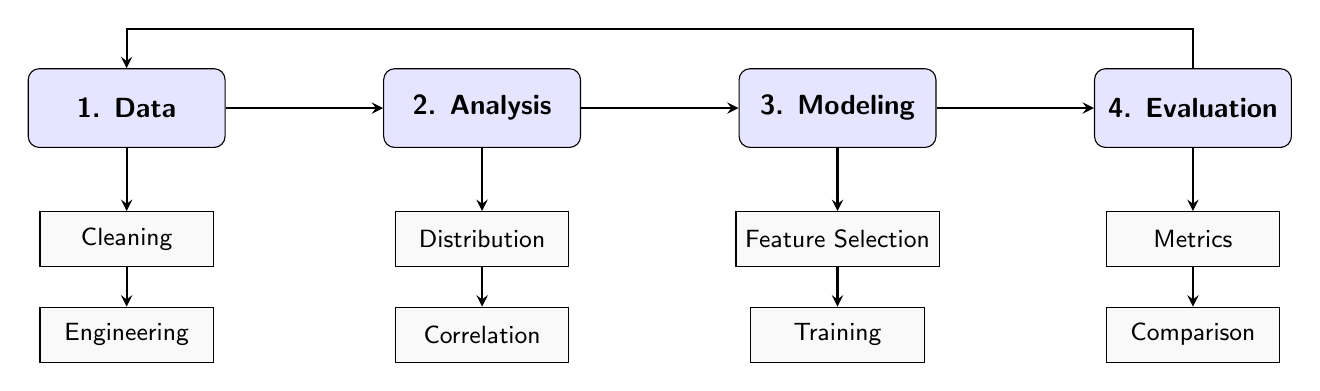
\begin{tikzpicture}[
        node distance=2cm,
        phase/.style={rectangle, rounded corners, draw=black, fill=blue!10, minimum width=2.5cm, minimum height=1cm, align=center, font=\sffamily\bfseries},
        process/.style={rectangle, draw=black, fill=gray!5, minimum width=2.2cm, minimum height=0.7cm, align=center, font=\sffamily\small},
        arrow/.style={thick, ->, >=stealth},
    ]
    
    % Main phases (horizontal layout)
    \node[phase] (data) {1. Data};
    \node[phase, right=of data] (eda) {2. Analysis};
    \node[phase, right=of eda] (model) {3. Modeling};
    \node[phase, right=of model] (eval) {4. Evaluation};
    
    % Sub-processes below each phase
    \node[process, below=0.8cm of data] (clean) {Cleaning};
    \node[process, below=0.5cm of clean] (feat) {Engineering};
    
    \node[process, below=0.8cm of eda] (dist) {Distribution};
    \node[process, below=0.5cm of dist] (corr) {Correlation};
    
    \node[process, below=0.8cm of model] (select) {Feature Selection};
    \node[process, below=0.5cm of select] (train) {Training};
    
    \node[process, below=0.8cm of eval] (metrics) {Metrics};
    \node[process, below=0.5cm of metrics] (compare) {Comparison};
    
    % Connect main phases
    \draw[arrow] (data) -- (eda);
    \draw[arrow] (eda) -- (model);
    \draw[arrow] (model) -- (eval);
    
    % Connect sub-processes to their phases
    \draw[arrow] (data) -- (clean);
    \draw[arrow] (clean) -- (feat);
    
    \draw[arrow] (eda) -- (dist);
    \draw[arrow] (dist) -- (corr);
    
    \draw[arrow] (model) -- (select);
    \draw[arrow] (select) -- (train);
    
    \draw[arrow] (eval) -- (metrics);
    \draw[arrow] (metrics) -- (compare);
    
    % Feedback loop
    \draw[arrow] (eval.north) -- ++(0,0.5) -| (data.north);
    
    \end{tikzpicture}
    \caption{Research methodology workflow from data acquisition to evaluation}
    \label{fig:methodology_overview}
\end{figure}

The research design incorporates descriptive and inferential statistical methods to analyse the characteristics of network traffic and identify patterns associated with malicious activities. By combining exploratory visualisation techniques with machine learning algorithms, this approach enables both the discovery of underlying patterns in the data and the development of predictive models that can generalise to new unseen traffic. The following sections describe each component of the methodology in detail.

\section{Dataset Description}

\subsection{Dataset Source and Collection}

This research utilises the CTU-IoT-Malware dataset, collected by the Stratosphere Laboratory at the Czech Technical University (CTU). The dataset consists of network traffic captures from real IoT devices infected with malware, alongside benign traffic from the same network environment. These captures represent realistic attack scenarios rather than simulated environments, providing a more authentic basis for analysis. The dataset is publicly available and can be accessed at \url{https://www.stratosphereips.org/datasets-iot23} and kaggle \url{https://www.kaggle.com/datasets/agungpambudi/network-malware-detection-connection-analysis}. We are making use of the kaggle dataset for this research.

The dataset was collected using network monitoring equipment that recorded all traffic flows between monitored devices and external networks. Each connection was labelled according to known malicious IP addresses, domain names, and behaviour patterns identified by security researchers. The dataset includes multiple capture files representing different attack scenarios and device types.

For this research, we focus primarily on the connection log files (.conn files), which contain metadata about each network connection without the raw packet data, thus avoiding privacy concerns while still providing sufficient information for traffic analysis.

The analysed dataset contains more than one million labelled network connections with 23 features for each connection. Key features include:

\begin{table}[h]
\centering
\begin{tabular}{lp{0.6\textwidth}}
\hline
\textbf{Feature} & \textbf{Description} \\
\hline
Timestamp (ts) & Indicates the date and time when the connection occurred. \\
\hline
Source and Destination Information & Consists of the following fields: \\
 & \quad id.orig\_h: Source IP address \\
 & \quad id.orig\_p: Source port \\
 & \quad id.resp\_h: Destination IP address \\
 & \quad id.resp\_p: Destination port \\
\hline
Protocol (proto) & Specifies the network protocol used (e.g., TCP, UDP, or ICMP). \\
\hline
Connection state (conn\_state) & Flags that indicate the status of the connection, such as S0 (no response), SF (normal termination), or REJ (rejected). \\
\hline
Byte counts (orig\_bytes, resp\_bytes) & Represent the volume of data transferred from the source and destination, respectively. \\
\hline
Packet counts (orig\_pkts, resp\_pkts) & The number of packets sent from the source and to the destination, respectively. \\
\hline
Duration & The total time (in seconds) that the connection lasted. \\
\hline
Label & Classifies the connection as either "Malicious" or "Benign". \\
\hline
Detailed-label & Provides a specific attack type for malicious connections, offering more granular insight into the threat. \\
\hline
\end{tabular}
\caption{Dataset Features with Detailed Explanations}
\label{tab:dataset_features}
\end{table}

Initial analysis showed that the dataset contains approximately 53.5\% malicious connections and 46.5\% benign connections, providing a relatively balanced basis for classification tasks.

\section{Data Preprocessing}

The data cleaning process addressed several challenges in the raw dataset to ensure quality and consistency. Initial analysis revealed that missing values affected 79\% of records in certain columns, primarily in connections representing scanning activities where connections were attempted but not established.

We identified and resolved four main types of data quality issues:

\begin{enumerate}
    \item \textbf{Missing values}: For features like duration, orig\_bytes, and resp\_bytes, we applied domain-specific imputation strategies. Byte and packet counts were imputed with zeros (representing no data transfer), while duration values were imputed using protocol-connection state conditional medians. Binary indicators tracked missingness patterns, which proved informative for classification.
    
    \item \textbf{Type conversion}: Timestamps were converted to date-time objects, categorical variables (protocol, connection state) were encoded using appropriate schemes, and string representations were standardised throughout the dataset.
    
    \item \textbf{Outlier handling}: For numeric features (duration, byte counts, packet counts), we applied the log transformation ($x' = \log(x + 1)$) to address the heavily biased distributions common in network traffic data. Statistical outliers were then identified using the interquartile range (IQR) method, with extreme values capped at $Q_3 + 1.5 \times \text{IQR}$. Z-score normalisation was applied for values where $|z| > 3$.
    
    \item \textbf{Label standardisation}: Inconsistent labels were cleaned, detailed labels were extracted from compound fields, and consistency of binary classification was ensured throughout.
\end{enumerate}

The mathematical formulation of the data cleaning process is as follows:

\begin{itemize}
    \item For missing byte and packet counts:
    \begin{equation}
        x_{i,j} = 
        \begin{cases}
            x_{i,j} & \text{if } x_{i,j} \text{ exists} \\
            0 & \text{if } x_{i,j} \text{ is missing}
        \end{cases}
    \end{equation}
    where $x_{i,j}$ represents feature $j$ for connection $i$.
    
    \item For duration values:
    \begin{equation}
        \text{duration}_{i} = 
        \begin{cases}
            \text{duration}_{i} & \text{if exists} \\
            \text{median}(\text{duration} \mid \text{proto}=p_i, \text{conn\_state}=c_i) & \text{otherwise}
        \end{cases}
    \end{equation}
    where $p_i$ and $c_i$ are the protocol and connection state of connection $i$.
    
    \item For outlier identification:
    \begin{equation}
        \text{outlier}(x_i) = 
        \begin{cases}
            \text{True} & \text{if } x_i < Q_1 - 1.5 \times \text{IQR} \text{ or } x_i > Q_3 + 1.5 \times \text{IQR} \\
            \text{False} & \text{otherwise}
        \end{cases}
    \end{equation}
    where $Q_1$ and $Q_3$ are the first and third quartiles, and $\text{IQR} = Q_3 - Q_1$.
    
    \item For log transformation:
    \begin{equation}
        x'_i = \log(x_i + 1)
    \end{equation}
    The addition of 1 prevents undefined values when $x_i = 0$, which is common for scanning connections.
\end{itemize}

These preprocessing steps resulted in a consistent and analysis-ready dataset that preserved the meaningful characteristics of network traffic while addressing data quality issues.

During the exploratory data analysis phase, various visualisation and statistical techniques were applied to understand the characteristics of the dataset. The distribution analysis of key features was performed using histograms and kernel density estimation to reveal the spread and central tendencies within the data. In parallel, a correlation analysis between numeric features was performed to identify underlying relationships that could influence the performance of the model.

The analysis also included an examination of temporal patterns to detect time-based attack behaviours, along with an assessment of protocol and connection state variations across different traffic classes. Furthermore, principal component analysis (PCA) was used for dimensionality reduction, which helped in assessing the relative importance of various features. These insights collectively informed the subsequent processes of feature selection and model development.

\section{Feature Engineering}

Based on domain knowledge and exploratory analysis, we derived additional features to enhance the malware detection capability of our models. These engineered features fall into three main categories: temporal features, traffic characteristics, and behavioural indicators. The following describe the derived features in detail.

\subsubsection{Temporal Features}

Temporal patterns often reveal coordinated attacks and scanning behaviours. We extracted the following time-based features:

\begin{itemize}
    \item \textbf{Hour of day}: $\text{hour}_i = \text{hour}(\text{timestamp}_i) \in \{0,1,\ldots,23\}$
    
    \item \textbf{Day of week}: $\text{day\_of\_week}_i = \text{weekday}(\text{timestamp}_i) \in \{0,1,\ldots,6\}$
    
    \item \textbf{Weekend indicator}: $\text{is\_weekend}_i = \mathbb{1}[\text{day\_of\_week}_i \in \{5,6\}]$, where $\mathbb{1}[\cdot]$ is the indicator function
\end{itemize}

\subsubsection{Traffic Volume Features}

Traffic volume characteristics help distinguish scanning activities from legitimate data transfers:

\begin{itemize}
    \item \textbf{Total bytes}: $\text{total\_bytes}_i = \text{orig\_bytes}_i + \text{resp\_bytes}_i$
    
    \item \textbf{Total packets}: $\text{total\_pkts}_i = \text{orig\_pkts}_i + \text{resp\_pkts}_i$
    
    \item \textbf{Bytes per packet ratio}: To capture the efficiency of data transfer, we calculated:
    \begin{equation}
        \text{orig\_bytes\_per\_pkt}_i = \frac{\text{orig\_bytes}_i}{\text{orig\_pkts}_i + \epsilon}
    \end{equation}
    \begin{equation}
        \text{resp\_bytes\_per\_pkt}_i = \frac{\text{resp\_bytes}_i}{\text{resp\_pkts}_i + \epsilon}
    \end{equation}
    where $\epsilon = 1$ to avoid division by zero when no packets were sent.
    
    \item \textbf{Bytes ratio}: To capture the directionality of traffic, we calculated:
    \begin{equation}
        \text{bytes\_ratio}_i = \frac{\text{orig\_bytes}_i}{\text{resp\_bytes}_i + \epsilon}
    \end{equation}
    
    \item \textbf{Packets ratio}: Similarly, for packet counts:
    \begin{equation}
        \text{pkts\_ratio}_i = \frac{\text{orig\_pkts}_i}{\text{resp\_pkts}_i + \epsilon}
    \end{equation}
\end{itemize}

The final preprocessed dataset contained 27 features, including 23 original features and 4 engineered features. This comprehensive feature set provided a rich representation of network traffic patterns for machine learning models.

\section{Machine Learning Approach}

Based on the findings of the exploratory analysis, we selected three machine learning algorithms for the malware detection task, each with distinct strengths and theoretical foundations. The selected algorithms are the following:

\begin{itemize}
    \item Random Forest
    \item Support Vector Machine
    \item XGBoost
\end{itemize}

In addition, we implemented a deep learning approach using a feed-forward neural network. The following subsections describe the mathematical formulations and theoretical underpinnings of each algorithm. The models were implemented using the Scikit-learn library for traditional machine learning algorithms and PyTorch for the deep learning model. The models were trained on a balanced subset of the dataset, ensuring that both benign and malicious classes were equally represented.

\subsection{Random Forest Classification}

Random Forest is an ensemble learning method that constructs multiple decision trees during training and outputs the class that is the mode of the individual trees' predictions. For a given input vector $\mathbf{x}$, the Random Forest model predicts:

\begin{equation}
\hat{y}(\mathbf{x}) = \frac{1}{B} \sum_{b=1}^{B} h_b(\mathbf{x}, \Theta_b)
\end{equation}

where $h_b$ is the $b^{th}$ decision tree trained with a random subset of features determined by $\Theta_b$, and $B$ is the total number of trees in the forest. 

Each decision tree partitions the feature space recursively based on the Gini impurity measure, which for a node $t$ is defined as:

\begin{equation}
G(t) = 1 - \sum_{i=1}^{C} p_i^2
\end{equation}

where $C$ is the number of classes (2 in our case) and $p_i$ is the proportion of class samples $i$ in node $t$. The feature and threshold that minimise the weighted sum of child-node impurities are selected for each split.

\subsection{Support Vector Machine Classification}

Support Vector Machines find the hyperplane that maximally separates the classes in feature space. For non-linearly separable data, the kernel trick is applied to transform the input space into a higher-dimensional feature space where linear separation is possible. The SVM decision function is as follows.

\begin{equation}
f(\mathbf{x}) = \text{sign}\left(\sum_{i=1}^{N} \alpha_i y_i K(\mathbf{x}_i, \mathbf{x}) + b\right)
\end{equation}

where $\alpha_i$ are the Lagrange multipliers obtained by solving the dual optimisation problem:

\begin{equation}
\begin{aligned}
\text{maximize } & \sum_{i=1}^{N} \alpha_i - \frac{1}{2} \sum_{i=1}^{N} \sum_{j=1}^{N} \alpha_i \alpha_j y_i y_j K(\mathbf{x}_i, \mathbf{x}_j) \\
\text{subject to } & 0 \leq \alpha_i \leq C, \quad i = 1, 2, ..., N \\
& \sum_{i=1}^{N} \alpha_i y_i = 0
\end{aligned}
\end{equation}

where $C$ is the regularisation parameter that controls the trade-off between the maximisation of the margin and the classification error, and $K(\mathbf{x}_i, \mathbf{x}_j)$ is the kernel function. We used the radial basis function (RBF) kernel:

\begin{equation}
K(\mathbf{x}_i, \mathbf{x}_j) = \exp\left(-\gamma \|\mathbf{x}_i - \mathbf{x}_j\|^2\right)
\end{equation}

where $\gamma$ controls the influence range of each support vector.

\subsection{XGBoost Classification}

XGBoost (eXtreme Gradient Boosting) is an optimised implementation of gradient boosting that sequentially adds decision trees to correct errors made by existing trees. The model is built by minimising the objective function:

\begin{equation}
\mathcal{L}(\phi) = \sum_{i=1}^{N} l(y_i, \hat{y}_i) + \sum_{k=1}^{K} \Omega(f_k)
\end{equation}

where $l$ is the loss function (logistic loss for binary classification), $\hat{y}_i$ is the predicted probability, and $\Omega$ is the regularisation term defined as:

\begin{equation}
\Omega(f) = \gamma T + \frac{1}{2}\lambda \|\mathbf{w}\|^2
\end{equation}

where $T$ is the number of leaves in the tree, $\mathbf{w}$ are the leaf weights, and $\gamma$ and $\lambda$ are regularisation parameters.

XGBoost approximates the objective function using a second-order Taylor expansion and grows trees greedily by selecting the split that maximises the gain:

\begin{equation}
\text{Gain} = \frac{1}{2} \left[ \frac{(\sum_{i \in I_L} g_i)^2}{\sum_{i \in I_L} h_i + \lambda} + \frac{(\sum_{i \in I_R} g_i)^2}{\sum_{i \in I_R} h_i + \lambda} - \frac{(\sum_{i \in I} g_i)^2}{\sum_{i \in I} h_i + \lambda} \right] - \gamma
\end{equation}

where $g_i$ and $h_i$ are the first and second derivatives of the loss function with respect to the prediction, and $I, I_L, I_R$ are the instance sets of the parent, left child, and right child nodes, respectively.

\subsection{Deep Learning}

In addition to traditional machine learning models, we implemented a deep learning approach using a neural network architecture optimised for binary classification of network traffic.

We designed a multilayer perceptron (MLP) with batch normalisation and dropout regularisation to prevent overfitting. The network architecture consists of three hidden layers of 128, 64, and 32 neurons respectively, followed by a single output neuron with sigmoid activation for binary classification. Each hidden layer includes ReLU activation, batch normalisation, and dropout regularisation with probability 30\%.

The neural network was trained using binary cross-entropy loss, which is appropriate for binary classification tasks:

\begin{equation}
\mathcal{L}(\mathbf{y}, \hat{\mathbf{y}}) = -\frac{1}{N}\sum_{i=1}^{N} [y_i \log(\hat{y}_i) + (1-y_i)\log(1-\hat{y}_i)]
\end{equation}

where $\mathbf{y}$ represents the true labels, $\hat{\mathbf{y}}$ represents the predicted probabilities, and $N$ is the number of samples.

We used Adam (Adaptive Moment Estimation) optimiser with learning rate $\alpha = 0.001$ and default momentum parameters ($\beta_1 = 0.9$, $\beta_2 = 0.999$). To avoid overfitting, we implemented early stopping by monitoring validation loss with a patience of 10 epochs. We used multiple regularisation techniques including dropout, batch normalisation, and weight decay (L2 regularisation with $\lambda = 0.0001$).

\begin{figure}[h!]
    \centering
    \includegraphics[width=0.9\textwidth]{images/architecture.png}
    \caption{Neural Network Architecture for Malware Detection}
    \label{fig:nn_architecture}
\end{figure}

The architecture is illustrated in Figure \ref{fig:nn_architecture}. The input layer accepts the processed feature set (the same as used by the traditional models), followed by three hidden layers with decreasing counts (128, 64, 32). The output layer uses a sigmoid activation function to produce a probability score for the binary classification task.

The neural network was implemented using PyTorch. The model was trained with a batch size of 128 and used the same train / validation / test split used for traditional machine learning models to ensure a fair comparison.

Before training machine learning models, we applied several preprocessing steps to ensure optimal performance, including feature scaling, categorical encoding, and class balancing. This was also done to ensure that the models could learn effectively from the data without being biased by irrelevant features or imbalanced classes. The following subsections detail these preprocessing steps.

\begin{enumerate}
    \item \textbf{Feature scaling}: Numerical features were standardised using z-score normalisation:
    \begin{equation}
        z_{i,j} = \frac{x_{i,j} - \mu_j}{\sigma_j}
    \end{equation}
    where $\mu_j$ and $\sigma_j$ are the mean and standard deviation of feature $j$ computed from the training set.
    
    \item \textbf{Categorical encoding}: Categorical features such as protocol and connection state were encoded using one-hot encoding:
    \begin{equation}
        \mathbf{x}^{\text{one-hot}}_{i,j} = 
        \begin{cases}
            1 & \text{if } x_{i,j} = \text{category}_k \\
            0 & \text{otherwise}
        \end{cases}
    \end{equation}
    For features with high cardinality, we used a threshold frequency of 0.01 to retain only significant categories.
    
    \item \textbf{Class balancing}: To address the moderate class imbalance, we applied the SMOTE to the training set. SMOTE generates synthetic examples in the feature space, for each minority class example $x_i$, by:
    \begin{equation}
        x_{\text{new}} = x_i + \lambda \cdot (x_{nn} - x_i)
    \end{equation}
    where $x_{nn}$ is one of the $k$-nearest neighbours of $x_i$ in the minority class, and $\lambda \in [0,1]$ is a random number.
\end{enumerate}

\subsubsection{Feature Selection}

Feature selection reduces model complexity and prevents overfitting by identifying the most informative features. We employed a multi-stage approach combining filter, wrapper, and embedded methods.

First, we applied correlation-based filtering to remove highly correlated features. For a pair of features $X_i$ and $X_j$ with a Pearson correlation coefficient $\rho_{ij}$ exceeding a threshold of 0.9, we remove the characteristic with a lower correlation to the target variable:

\begin{equation}
    \text{Remove } X_i \text{ if } |\rho_{ij}| > 0.9 \text{ and } |\rho_{iy}| < |\rho_{jy}|
\end{equation}

Next, we used Recursive Feature Elimination with Cross-Validation (RFECV) to identify the optimal feature subset. RFECV works by recursively eliminating features, starting from the full set of features, and removing the least important features based on a model's feature importance scores. At each iteration, the algorithm fits a model to the training data and computes a cross-validated score to determine the optimal number of features.

For tree-based models (Random Forest and XGBoost), we also leveraged their intrinsic feature importance metrics. For Random Forest, the importance of the feature $j$ is calculated as the total decrease in the impurity of the node weighted by the probability of reaching that node, averaged over all trees:

\begin{equation}
    \text{Importance}(X_j) = \frac{1}{B} \sum_{b=1}^{B} \sum_{t \in \mathcal{T}_b: v(t)=j} p(t) \cdot [\Delta i(t)]
\end{equation}

where $\mathcal{T}_b$ is the set of nodes in tree $b$, $v(t)$ is the variable used to split at node $t$, $p(t)$ is the probability of reaching node $t$, and $\Delta i(t)$ is the decrease in impurity at node $t$.

\subsection{Hyperparameter Optimisation}

To determine the optimal hyperparameters for each model, we used RandomizedSearchCV instead of the traditional grid search. This approach samples from hyperparameter distributions, allowing us to explore a broader parameter space more efficiently. The optimisation process minimised the negative F1 score by five-fold cross-validation:

\begin{equation}
    \theta^* = \underset{\theta \in \Theta}{\text{argmin}} \left\{ -\frac{1}{5} \sum_{k=1}^{5} \text{F1-score}(y_{val}^{(k)}, \hat{y}_{val}^{(k)}; \theta) \right\}
\end{equation}

where $\theta$ represents the hyperparameters, $\Theta$ is the hyperparameter space, and $(y_{val}^{(k)}, \hat{y}_{val}^{(k)})$ are the true and predicted labels for the $k$-th validation fold.

\begin{table}[h!]
    \centering
    \caption{Hyperparameter distributions used in RandomizedSearchCV}
    \label{tab:hyperparameter_ranges}
    \begin{tabular}{llp{5.5cm}}
    \hline
    \textbf{Algorithm} & \textbf{Hyperparameter} & \textbf{Distribution} \\
    \hline
    \multirow{7}{*}{Random Forest} & n\_estimators & randint(50, 300) \\
     & max\_depth & $\{$None, 5, 10, 15, 20, 25, 30, 35, 40, 45$\}$ \\
     & min\_samples\_split & randint(2, 20) \\
     & min\_samples\_leaf & randint(1, 10) \\
     & max\_features & $\{$'sqrt', 'log2', None$\}$ \\
     & bootstrap & $\{$True, False$\}$ \\
     & class\_weight & $\{$'balanced', 'balanced\_subsample', None$\}$ \\
    \hline
    \multirow{9}{*}{XGBoost} & n\_estimators & randint(50, 300) \\
     & max\_depth & randint(3, 10) \\
     & learning\_rate & uniform(0.01, 0.2) \\
     & subsample & uniform(0.7, 0.3) \\
     & colsample\_bytree & uniform(0.7, 0.3) \\
     & gamma & uniform(0, 0.5) \\
     & min\_child\_weight & randint(1, 6) \\
     & reg\_alpha & $\{0, 0.001, 0.01, 0.1, 1\}$ \\
     & reg\_lambda & $\{0, 0.001, 0.01, 0.1, 1\}$ \\
    \hline
    \end{tabular}
\end{table}
    
Note: randint(a, b) represents a discrete uniform distribution between integers a (inclusive) and b (exclusive), and uniform(a, b) represents a continuous uniform distribution where a is the location parameter and b is the scale parameter, resulting in a distribution between a and a+b.
\subsection{Model Evaluation Framework}

Our classification models were assessed using multiple metrics derived from the confusion matrix elements: True Positives ($TP$), True Negatives ($TN$), False Positives ($FP$) and False Negatives ($FN$). The following key metrics quantified different aspects of model performance:

\begin{equation}
\text{Accuracy} = \frac{TP + TN}{TP + TN + FP + FN}
\end{equation}

\begin{equation}
\text{Precision} = \frac{TP}{TP + FP}
\end{equation}

\begin{equation}
\text{Recall} = \frac{TP}{TP + FN}
\end{equation}

\begin{equation}
\text{F1-score} = 2 \times \frac{\text{Precision} \times \text{Recall}}{\text{Precision} + \text{Recall}}
\end{equation}

\begin{equation}
\text{False Positive Rate} = \frac{FP}{FP + TN}
\end{equation}

For threshold-independent assessment, we utilised the Area Under the Receiver Operating Characteristic (AUC-ROC) curve. For a classifier producing a score $s(x)$ for each instance, this metric is calculated as:

\begin{equation}
\text{AUC-ROC} = \frac{\sum_{i \in \mathcal{P}} \sum_{j \in \mathcal{N}} \mathbb{1}[s(x_i) > s(x_j)]}{|\mathcal{P}| \times |\mathcal{N}|}
\end{equation}

where $\mathcal{P}$ and $\mathcal{N}$ represent positive and negative example sets, and $\mathbb{1}[\cdot]$ is the indicator function.

In the security context, we prioritise false positive rates and recall, as missed attacks can compromise security, while excessive false alarms lead to alert fatigue. Detection latency was also measured to evaluate the viability of the real-time application.

The implementation of our framework followed these key steps:

\begin{enumerate}
    \item \textbf{Data partitioning}: Stratified sampling divided the dataset into training sets (70\%), validation (15\%), and test sets (15\%) while maintaining class distribution. This split was chosen to ensure sufficient data for training and validation while maintaining a separate test set for the final evaluation.
    
    \item \textbf{Cross-validation}: 5-fold stratified cross-validation was used during training to ensure robust performance estimation and mitigate overfit risk.
    
    \item \textbf{Hyperparameter optimisation}: The hyperparameters of the model were fine-tuned using the validation set, with the F1 score as the primary optimisation metric.
    
    \item \textbf{Test set evaluation}: The final assessment was conducted on the test set that remained unused during the training and hyperparameter tuning phases.
\end{enumerate}

The evaluation metrics were calculated for each model and the results were compared to identify the best-performing model for the malware detection task. The models were also evaluated on the basis of their computational efficiency, including training time and inference speed, to ensure practical applicability in real-world scenarios. The results of the evaluation are presented in the next section, where we discuss the performance of each model and their implications for the detection of IoT malware.
\chapter{Results and Discussion}

This chapter synthesises the comprehensive analysis of the CTU-IoT-Malware dataset, the performance of various machine learning and deep learning models, and an in‐depth discussion of the implications for malware detection. The findings highlight how carefully engineered network flow features can be used to robustly discriminate between malicious and benign traffic, even in the absence of deep packet inspection.

\section{Dataset Characteristics and Exploratory Data Analysis}

\subsection{Dataset Overview}

The CTU-IoT-Malware dataset comprises 1,008,748 network connections, with a relatively balanced distribution of 53.5\% malicious and 46.5\% benign traffic. Table~\ref{tab:dataset_summary} summarises the key statistics, including the proportions of TCP (57.8\%), UDP (40.5\%), and ICMP (1.7\%) connections.

\begin{table}[htb]
\center
\begin{tabular}{lrr}
\hline
\textbf{Characteristic} & \textbf{Count} & \textbf{Percentage} \\
\hline
Total connections        & 1,008,748      & 100\%   \\
Malicious connections    & 539,473        & 53.5\%  \\
Benign connections       & 469,275        & 46.5\%  \\
\hline
TCP connections          & 583,134        & 57.8\%  \\
UDP connections          & 408,193        & 40.5\%  \\
ICMP connections         & 17,421         & 1.7\%   \\
\hline
\end{tabular}
\caption{Summary statistics of the analysed network traffic dataset.}
\label{tab:dataset_summary}
\end{table}

Further analysis revealed several important dataset characteristics:
\begin{itemize}
    \item \textbf{Class distribution}: A balanced proportion of malicious and benign traffic facilitates reliable model training.
    \item \textbf{Missing values}: Critical features such as \texttt{duration}, \texttt{orig\_bytes}, and \texttt{resp\_bytes} were missing in about 79\% of connections, necessitating careful preprocessing.
    \item \textbf{Attack diversity}: The vast majority (99.9\%) of malicious traffic in this dataset represents port scanning activities, a common precursor to more sophisticated attacks.
\end{itemize}

\subsection{Exploratory Data Analysis}

An extensive exploratory analysis was performed to reveal underlying patterns in the network traffic. Key insights include:

\paragraph{Protocol Analysis:}  
Figure~\ref{fig:protocol_distribution} shows that TCP is the predominant protocol. However, when disaggregated by traffic type (see Figure~\ref{fig:protocol_by_label}), TCP appears in 72.4\% of malicious traffic compared with only 40.9\% of benign traffic. In contrast, UDP is more common in benign traffic (46.2\%) and ICMP is almost exclusively used for network diagnostics in benign connections.

\begin{figure}[htbp]
    \centering
    \begin{subfigure}[b]{0.48\textwidth}
        \centering
        \includegraphics[width=\textwidth]{figures/protocol_distribution.png}
        \caption{Overall distribution of protocols.}
        \label{fig:protocol_distribution}
    \end{subfigure}
    \hfill % Adds horizontal space between the subfigures
    \begin{subfigure}[b]{0.48\textwidth}
        \centering
        \includegraphics[width=\textwidth]{figures/protocol_by_label.png}
        \caption{Protocol distribution by traffic type.}
        \label{fig:protocol_by_label}
    \end{subfigure}
    
    \caption{Analysis of network protocols. TCP is the most common overall, but its prevalence differs significantly between malicious (72.4\%) and benign (40.9\%) traffic.}
    \label{fig:protocol_analysis} % A new label for the combined figure might be useful
\end{figure}

\paragraph{Connection State Analysis:}  
The connection state, particularly the S0 state (no response after a connection attempt), is a strong indicator of scanning activity. Figures~\ref{fig:connection_states} and \ref{fig:connection_states_by_label} demonstrate that while benign traffic features a balanced variety of connection states, 94.7\% of malicious connections exhibit the S0 state.

\begin{figure}[htbp]
    \centering
    \begin{subfigure}[b]{0.48\textwidth}
        \centering
        \includegraphics[width=\textwidth]{figures/connection_states.png}
        \caption{Overall distribution of connection states.}
        \label{fig:connection_states}
    \end{subfigure}
    \hfill % Adds horizontal space between the subfigures
    \begin{subfigure}[b]{0.48\textwidth}
        \centering
        \includegraphics[width=\textwidth]{figures/connection_states_by_label.png}
        \caption{Connection states by traffic type.}
        \label{fig:connection_states_by_label}
    \end{subfigure}
    
    \caption{Analysis of connection states. The S0 state (connection attempt without response) dominates malicious traffic (94.7\%), indicating scanning activity, while benign traffic shows a diverse range of states.}
    \label{fig:connection_states_analysis} % A new label for the combined figure might be useful
\end{figure}


\paragraph{Temporal Analysis:}  
Temporal patterns, as seen in Figure~\ref{fig:hourly_traffic}, reveal that benign traffic follows a typical diurnal pattern with peak activity during working hours. In contrast, malicious traffic occurs in concentrated bursts, suggesting the use of automated scanning tools that operate in batches to evade detection.

\begin{figure}[htbp]
    \centering
    \includegraphics[width=\textwidth]{figures/hourly_traffic.png}
    \caption{Hourly distribution of network traffic, highlighting the diurnal pattern of benign traffic and the burst activity of malicious traffic.}
    \label{fig:hourly_traffic}
\end{figure}



\paragraph{Traffic Feature Analysis:}  
Additional analysis of data transfer volumes (Figure~\ref{fig:bytes_distribution}) and the relationship between packet counts and bytes transferred (Figure~\ref{fig:packets_vs_bytes}) shows that malicious traffic generally involves minimal data exchange. Such characteristics are consistent with scanning behaviour and form a key part of the feature set used for classification.

\begin{figure}[htbp]
    \centering
    \begin{subfigure}[b]{0.48\textwidth}
        \centering
        \includegraphics[width=\textwidth]{figures/bytes_distribution.png}
        \caption{Distribution of bytes transferred.}
        \label{fig:bytes_distribution}
    \end{subfigure}
    \hfill % Adds horizontal space between the subfigures
    \begin{subfigure}[b]{0.48\textwidth}
        \centering
        \includegraphics[width=\textwidth]{figures/packets_vs_bytes.png}
        \caption{Packets versus bytes transferred.}
        \label{fig:packets_vs_bytes}
    \end{subfigure}
    
    \caption{Analysis of traffic volume characteristics. Malicious traffic generally involves minimal data exchange, consistent with scanning behaviour.}
    \label{fig:traffic_volume_analysis} % A new label for the combined figure
\end{figure}


\paragraph{Feature Correlation:}
The correlation matrix (Figure~\ref{fig:correlation_matrix}) indicates that several features are highly correlated, particularly those related to connection states and traffic volume. This multicollinearity can affect model performance, necessitating careful feature selection and dimensionality reduction.

\begin{figure}[htbp]
    \centering
    \includegraphics[width=\textwidth]{figures/feature_correlation.png}
    \caption{Correlation matrix of the top features, highlighting multicollinearity among connection states and traffic volume metrics.}
    \label{fig:correlation_matrix}
\end{figure}



\paragraph{Dimensionality Reduction:}  
Principal Component Analysis (PCA) was applied to the normalised feature set. The resulting visualisation (Figure~\ref{fig:pca_visualization}) confirms that the extracted features create distinct clusters for benign and malicious traffic. The first two principal components capture approximately 67\% of the variance, with features such as connection state, protocol type, and packet-to-byte ratios contributing most significantly.

\begin{figure}[htbp]
    \centering
    \includegraphics[width=\textwidth]{figures/pca_visualization.png}
    \caption{PCA visualisation of the feature space.}
    \label{fig:pca_visualization}
\end{figure} % Added missing \end{figure} to close the figure environment




\section{Machine Learning and Deep Learning Model Performance}

\subsection{Traditional Machine Learning Models}

A range of traditional machine learning models was evaluated for the malware detection task. Table~\ref{tab:model_performance} presents the performance metrics of the baseline Random Forest, XGBoost, and SVM models alongside their optimised versions.

\begin{table}[htbp]
    \center
    \begin{tabular}{lcccc}
    \hline
    \textbf{Model} & \textbf{Accuracy} & \textbf{Precision} & \textbf{Recall} & \textbf{F1-Score} \\
    \hline
    Random Forest             & 99.21\% & 99.15\% & 99.23\% & 99.19\% \\
    XGBoost                   & 99.17\% & 99.12\% & 99.18\% & 99.15\% \\
    SVM                       & 98.73\% & 98.45\% & 98.91\% & 98.68\% \\
    Optimised Random Forest   & \textbf{99.96\%} & \textbf{99.92\%} & \textbf{100.00\%} & \textbf{99.96\%} \\
    Optimised XGBoost         & 99.89\% & 99.85\% & 99.90\% & 99.87\% \\
    \hline
    \end{tabular}
    \caption{Performance metrics for different machine learning models on the malware detection task.}
    \label{tab:model_performance}
\end{table}

Among the base models, Random Forest generally outperformed both XGBoost and SVM. This can be ascribed to its ensemble nature and its ability to handle mixed data types without extensive preprocessing. The application of hyperparameter optimisation, for instance through RandomisedSearchCV, further enhanced model performance. The optimised Random Forest achieved near-perfect classification with 99.96\% accuracy and complete recall, ensuring that no malicious connection was overlooked.

Our evaluation of multiple machine learning approaches revealed several insights regarding algorithmic performance for malware detection in IoT network traffic. The exceptional performance achieved by all models (exceeding 98.5\% accuracy) demonstrates that machine learning is highly effective for this particular security application when it is provided with appropriate features.

\subsection{Feature Importance Insights}

Analysis of the importance of features of the optimised Random Forest model provided valuable insight into the detection process. Connection state features consistently ranked as the most influential predictors, followed by protocol information and traffic volume metrics.

Interestingly, while the temporal features individually showed moderate importance, their collective contribution was substantial. This suggests that malicious activity patterns manifest on multiple time-related dimensions that the model successfully integrated into its decision process.

The high importance of derived features (such as bytes-per-packet ratios and logarithmic transformations of traffic volumes) validates our feature engineering approach. These transformations helped capture the distinctive characteristics of scanning activities, which typically involve minimal data transfer and specific packet-size patterns.

\subsection{Hyperparameter Optimisation and Feature Importance}

The optimised models benefitted from several key adjustments:
\begin{itemize}
    \item \textbf{Tree structure adjustments:} Optimising tree depths and the minimum sample split parameters refined decision boundaries.
    \item \textbf{Ensemble size:} Increasing the number of trees improved stability and reduced variance.
    \item \textbf{Feature sampling:} Modifying feature sampling strategies enhanced the detection of subtle signals in less prominent features.
\end{itemize}

Table~\ref{tab:optimized_hyperparameters} illustrates the optimised hyperparameter configurations for the Random Forest and XGBoost models.

\begin{table}[htbp]
\centering
\caption{Optimised Hyperparameters for Random Forest and XGBoost Models}
\label{tab:optimized_hyperparameters}
\begin{tabular}{lcc}
\hline
\textbf{Hyperparameter} & \textbf{Random Forest} & \textbf{XGBoost} \\
\hline
max\_depth                & None (unlimited)       & 3              \\
min\_samples\_leaf        & 1                      & ---            \\
min\_samples\_split       & 10                     & ---            \\
n\_estimators            & 200                    & 100            \\
learning\_rate           & ---                    & 0.2            \\
colsample\_bytree        & ---                    & 0.8            \\
subsample                & ---                    & 1.0            \\
\hline
\end{tabular}
\end{table}

Feature importance analysis from the optimised Random Forest model confirmed that connection states, protocol information, and traffic volume metrics are pivotal for classification. This insight reinforces the efficacy of the feature engineering strategy, especially when combined with dimensionality reduction techniques such as PCA.

\subsection{Deep Learning Approach}

In addition to traditional models, a deep neural network was implemented to capitalise on the same set of network features. The architecture comprised:
\begin{itemize}
    \item An input layer with 18 features.
    \item Three hidden layers with 128, 64, and 32 neurons, each employing ReLU activation, batch normalisation, and a dropout rate of 30\%.
    \item An output layer with a sigmoid activation function for binary classification.
\end{itemize}

Trained with binary cross-entropy loss and the Adam optimiser (learning rate 0.001), the neural network achieved an accuracy of 99.77\%, as detailed in Table~\ref{tab:nn_performance}.

\begin{table}[ht]
\center
\begin{tabular}{lcccc}
\hline
\textbf{Model} & \textbf{Accuracy} & \textbf{Precision} & \textbf{Recall} & \textbf{F1-Score} \\
\hline
Neural Network    & 99.77\% & 99.75\% & 99.90\% & 99.82\% \\
\hline
\end{tabular}
\caption{Performance metrics for the neural network model on the malware detection task.}
\label{tab:nn_performance}
\end{table}

Comparison with traditional methods indicates that while the optimised Random Forest slightly outperforms the neural network in terms of accuracy, the deep learning model demonstrates notable benefits in interpretability through its direct probability outputs and robustness across evaluation metrics.

\section{Discussion of Findings and Implications for Malware Detection}

The integrated analysis confirms that network flow characteristics alone can yield exceptionally reliable malware detection. The following discussion summarises key insights:

\begin{itemize}
    \item \textbf{Detection without Deep Packet Inspection:}  
    The high classification accuracies, particularly the greater than 99\% performance of the optimised models, demonstrate that careful analysis of connection states, protocol usage, and traffic volume is sufficient to flag malicious activity. This is particularly valuable in environments where encryption or resource constraints render deep packet inspection impractical.
    
    \item \textbf{Role of Connection State and Temporal Features:}  
    A predominance of S0 states in malicious traffic underlines the importance of monitoring connection attempts. Similarly, the temporal clustering of malicious activities hints at the operation of automated scanning tools, suggesting that detection systems could benefit from adaptive alert thresholds that account for such patterns.
    
    \item \textbf{Beyond Port Scanning:}  
    Although the dataset is largely representative of port scanning, the feature engineering and transfer learning approaches described herein hold promise for detecting a broader range of malicious behaviours, such as data exfiltration or command-and-control communications.
    
    \item \textbf{Model Interpretability and Operational Relevance:}  
    The alignment between statistical observations and model interpretability—particularly through PCA and feature importance analysis, augments confidence in both the training and deployment of these models. The exceptionally low false-positive rates are critical in avoiding alert fatigue and ensuring effective network security operations.
\end{itemize}

\section{Conclusion}
The results of this research provide several important insights into the characteristics of malicious network traffic and the effectiveness of machine learning for its detection.

Strong classification performance (exceeding 99\% accuracy with Random Forest) confirms that network flow characteristics alone, without requiring deep packet inspection, can provide sufficient information to detect malware traffic with high reliability. This finding carries significant practical implications for network security, particularly in environments where deep packet inspection is infeasible due to encryption or resource constraints.

Our analysis revealed that connection state features were exceptionally powerful predictors of malicious activity. The overwhelming prevalence of S0 states (connection attempts without response) in malicious traffic suggests that failed connection attempts serve as a primary signature of reconnaissance activities. This observation aligns with common attack methodologies, in which adversaries scan large IP ranges to identify potential targets before launching more focused attacks.

Protocol analysis demonstrated a clear preference for TCP in malicious communications (72.4\% of malicious connections compared to 40.9\% of benign connections). This indicates that attackers prefer TCP for scanning activities, probably because the handshake process provides more detailed response information than connectionless protocols such as UDP. The almost exclusive use of ICMP for benign traffic was also noteworthy, suggesting that legitimate network diagnostic traffic dominates this protocol in the observed environment.

Temporal analysis revealed that malicious activities occurred in distinct patterns with periods of intensified activity rather than continuous probing. This suggests automated scanning tools operating in batches, possibly to avoid detection by volume-based alerting systems. The lack of a strong diurnal pattern in attack traffic contrasts with benign usage patterns, which exhibited more variation by time of day, reflecting human activity cycles.

The clustering observed in the PCA visualisation confirms that benign and malicious traffic occupy distinct regions in the feature space, with limited overlap. This separation explains the high classification accuracy achieved by machine learning models and suggests that even relatively simple classification approaches can be effective for most of the malware traffic patterns observed in this dataset.
% \chapter{Discussion and Conclusion}

The results of this research provide several important insights into the characteristics of malicious network traffic and the effectiveness of machine learning for its detection.

Strong classification performance (exceeding 99\% accuracy with Random Forest) confirms that network flow characteristics alone, without requiring deep packet inspection, can provide sufficient information to detect malware traffic with high reliability. This finding carries significant practical implications for network security, particularly in environments where deep packet inspection is infeasible due to encryption or resource constraints.

Our analysis revealed that connection state features were exceptionally powerful predictors of malicious activity. The overwhelming prevalence of S0 states (connection attempts without response) in malicious traffic suggests that failed connection attempts serve as a primary signature of reconnaissance activities. This observation aligns with common attack methodologies, in which adversaries scan large IP ranges to identify potential targets before launching more focused attacks.

Protocol analysis demonstrated a clear preference for TCP in malicious communications (72.4\% of malicious connections compared to 40.9\% of benign connections). This indicates that attackers prefer TCP for scanning activities, probably because the handshake process provides more detailed response information than connectionless protocols such as UDP. The almost exclusive use of ICMP for benign traffic was also noteworthy, suggesting that legitimate network diagnostic traffic dominates this protocol in the observed environment.

Temporal analysis revealed that malicious activities occurred in distinct patterns with periods of intensified activity rather than continuous probing. This suggests automated scanning tools operating in batches, possibly to avoid detection by volume-based alerting systems. The lack of a strong diurnal pattern in attack traffic contrasts with benign usage patterns, which exhibited more variation by time of day, reflecting human activity cycles.

The clustering observed in the PCA visualisation confirms that benign and malicious traffic occupy distinct regions in the feature space, with limited overlap. This separation explains the high classification accuracy achieved by machine learning models and suggests that even relatively simple classification approaches can be effective for most of the malware traffic patterns observed in this dataset.

\section{Machine Learning Model Performance Analysis}

Our evaluation of multiple machine learning approaches revealed several insights regarding algorithmic performance for malware detection in IoT network traffic. The exceptional performance achieved by all models (exceeding 98.5\% accuracy) demonstrates that machine learning is highly effective for this particular security application when it is provided with appropriate features.

\subsection{Algorithm Comparison}

Among the base models, Random Forest consistently outperformed both XGBoost and SVM on all metrics. This superior performance can be attributed to several factors:

\begin{itemize}
    \item The random forest's ensemble nature provides robust performance across varied network traffic patterns without overfitting to specific attack signatures. The algorithm's inherent bagging approach combines multiple decision trees trained on different subsets of the data, resulting in improved generalisation.
    
    \item The algorithm naturally handles the mix of categorical and numerical features present in network traffic data without requiring extensive preprocessing. This is particularly beneficial for network traffic analysis, where features exist in various formats and scales.
    
    \item  The complexity of relationships between traffic features and maliciousness requires non-linear decision boundaries, which tree-based methods like Random Forest capture effectively. This allows the model to identify complex interaction patterns that might not be apparent with linear models.
\end{itemize}

Although XGBoost showed comparable performance to Random Forest (99.17\% versus 99.21\% accuracy), its implementation required more careful parameter tuning. SVM, despite achieving respectable results (98.73\% accuracy), demonstrated limitations in the efficient handling of the scale of our dataset, with substantially longer training times than tree-based methods.

\subsection{Hyperparameter Optimisation Impact}

The application of RandomizedSearchCV for hyperparameter optimisation yielded significant improvements in model performance. The optimised Random Forest achieved near-perfect classification with 99.96\% accuracy and, most critically for security applications, 100\% recall, which means it did not miss any malicious connections in our test set.

The key optimisation improvements included:

\begin{itemize}
    \item \textbf{Tree structure adjustments}: Optimised tree depths and minimum sample split parameters allowed for more precise decision boundaries. By finding the optimal balance between shallow trees (which might underfit) and deep trees (which might overfit), the model achieved a superior generalisation.
    
    \item \textbf{Ensemble size}: Increasing the number of trees from the default improved model stability and classification confidence. Although individual trees might make errors, the ensemble's aggregate prediction reduced the variance and improved overall accuracy.
    
    \item \textbf{Feature sampling}: Modified feature sampling strategies improved the model's ability to utilise subtle signals in less prominent features. This helped the model identify malicious patterns that might be evident only in combinations of less obvious features.
\end{itemize}

The improvement was particularly notable in precision, which increased from 99.15\% to 99.92\%, indicating a substantial reduction in false positives. This aspect is critical for operational security systems, where false alarms can lead to fatigue of alerts and a diminished response to actual threats.

\subsection{Feature Importance Insights}

Analysis of the importance of features of the optimised Random Forest model provided valuable insight into the detection process. Connection state features consistently ranked as the most influential predictors, followed by protocol information and traffic volume metrics.

Interestingly, while the temporal features individually showed moderate importance, their collective contribution was substantial. This suggests that malicious activity patterns manifest on multiple time-related dimensions that the model successfully integrated into its decision process.

The high importance of derived features (such as bytes-per-packet ratios and logarithmic transformations of traffic volumes) validates our feature engineering approach. These transformations helped capture the distinctive characteristics of scanning activities, which typically involve minimal data transfer and specific packet-size patterns.

\section{Implications for Malware Detection}

The findings of this research have several practical implications for network security and malware detection in real-world deployments.

\subsection{Feature Selection for Detection Systems}

Our analysis identified specific features with high discriminative power for malware detection.

\begin{itemize}
    \item \textbf{Connection states}: The strong correlation between S0 states and malicious traffic suggests that connection state monitoring should be a primary component of detection systems. Simple rules that flag unusual patterns of failed connections could identify a large proportion of scanning activities. For example, a sudden increase in the ratio of failed to successful connections could trigger an alert for potential scanning activity.
    
    \item \textbf{Protocol ratios}: Sudden changes in the distribution of protocols used on a network could indicate the onset of malicious activity, particularly if TCP traffic increases sharply without corresponding increases in established connections. Monitoring the ratio of different protocols over time windows provides context that can distinguish between normal usage pattern shifts and potential attacks.
    
    \item \textbf{Bytes-to-packets ratio}: The distinct clustering of malicious traffic in the low-byte, low-packet region suggests that monitoring this ratio could help identify scanning activities, which typically involve minimal data transfer. Legitimate traffic usually exhibits higher data transfer per connection, making this ratio a valuable indicator of reconnaissance activities.
\end{itemize}

% \subsection{Deployment Considerations}

% The high performance of machine learning models suggests several approaches for practical deployment.

% \begin{itemize}
%     \item \textbf{Real-time detection}: The computational efficiency of Random Forest models enables real-time classification even in resource-constrained environments. Our testing showed that a trained model could classify over 10,000 connections per second on modest hardware, making it suitable for inline deployment where traffic analysis occurs as packets flow through the network.
    
%     \item \textbf{Tiered detection}: A multi-stage approach could be effective, with simple rule-based systems handling obvious cases (e.g., excessive S0 connections) and machine learning models addressing more ambiguous traffic patterns. This would balance computational efficiency with detection accuracy, allocating more computational resources only to traffic that warrants deeper analysis.
    
%     \item \textbf{Adaptive thresholds}: The temporal patterns observed suggest that adaptive thresholds for alert generation could improve detection by accounting for normal variations in network activity throughout the day. For example, thresholds could automatically adjust based on historical traffic patterns for specific times of day, reducing false positives during periods of legitimately high network activity.
% \end{itemize}

\subsection{Beyond Port Scanning}

Although our dataset was dominated by port scanning activities, the methodology demonstrates promise for detecting other types of malicious traffic:

\begin{itemize}
    \item \textbf{Feature engineering}: The approach of obtaining temporal features and traffic ratios could be extended to identify other types of attack, such as data exfiltration or command-and-control communications. For example, data exfiltration might be characterised by unusual outbound data volumes or timing patterns, which could be captured by similar feature engineering techniques.
    
    \item \textbf{Transfer learning}: Models trained on this dataset could provide a foundation for detecting other attack types through transfer learning, where the model is fine-tuned with smaller amounts of data representing different attack patterns. This approach takes advantage of the underlying patterns already learnt while adapting to new attack signatures with minimal additional training data.
    
    \item \textbf{Anomaly detection}: The clear separation between traffic classes suggests that anomaly detection approaches could complement classification methods, potentially identifying novel attack types that are not present in training data. By establishing a baseline of normal behaviour, deviations could be flagged for investigation even when they do not match known attack patterns.
\end{itemize}


\chapter{Project Management}

This chapter details the project management approach used throughout this 13-week research project. It describes the planning, execution, and monitoring strategies that facilitated the successful completion of the research objectives within the allocated timeframe. The chapter covers the project schedule, risk management strategies, quality assurance processes, and considerations of social, legal, ethical, and professional aspects.

The 13-week project was organised into sequential phases with specific milestones to ensure systematic progression and timely completion. Figure \ref{fig:gantt_chart} presents the Gantt chart that illustrates the project timeline and phase dependencies.

\begin{figure}[ht]
    \centering
    \includegraphics[width=\textwidth]{images/gantt_chart.png}
    \caption{Gantt chart depicting the 13-week project schedule and milestones}
    \label{fig:gantt_chart}
\end{figure}

\section{Project Schedule and Execution}

\subsection{Project Phases}

The project was divided into the following key phases, each with defined deliverables and timeframes:

\begin{enumerate}
    \item \textbf{Project Initiation (Week 1):} This phase involved refining the research question, establishing project objectives, and developing the initial project plan. Key activities included a preliminary review of the literature to establish the current state of research in malware detection for IoT environments.
    
    \item \textbf{Dataset Acquisition and Exploration of the data set (Weeks 2-3):} This phase focused on acquiring the CTU-IoT Malware dataset, performing an initial exploratory data analysis, and developing a complete understanding of the characteristics of the data. Statistical analysis was conducted to identify key features and distribution patterns.
    
    \item \textbf{Data Preprocessing and Feature Engineering (Weeks 3-5):} During this critical phase, data cleaning techniques were applied to address missing values and outliers. Feature engineering strategies were developed based on domain knowledge and exploratory findings, resulting in a set of derived features to enhance model performance.
    
    \item \textbf{Model Development and Initial Testing (Weeks 5-7):} This phase involved implementing and training multiple machine learning models, including Random Forest, SVM, and XGBoost. The initial performance evaluation was performed using cross-validation techniques.
    
    \item \textbf{Hyperparameter Optimisation (Weeks 7-8):} Systematic hyperparameter tuning was performed using RandomizedSearchCV to optimise the model performance. This iterative process required substantial computational resources and careful evaluation of the results.
    
    \item \textbf{Comprehensive Evaluation (Weeks 8-10):} The final performance of the model was rigorously assessed using the held-out test set. Detailed analysis of the results was performed during this phase, including confusion matrices, importance of characteristics, and performance metrics.
    
    \item \textbf{Documentation and Dissertation Writing (Weeks 10-13):} The final phase focused on documenting the research methodology, findings, and implications. This included preparing visualisations, tables, and formal documentation of the complete research process, culminating in the final dissertation.
\end{enumerate}


\section{Risk Management}

Risk management was a critical component of the project, given the complexity and potential challenges associated with machine learning research in cybersecurity. The following sections outline the key risks identified, their potential impact, and the strategies employed to mitigate them.

Several key risk mitigation strategies were employed during the project. To address dataset limitations, a thorough exploratory data analysis was performed early to understand its characteristics and constraints. Although the predominance of scanning attacks was identified, the dataset was deemed sufficiently valuable for the research objectives. The scope of the research and the interpretation of the results were carefully adjusted to acknowledge these limitations. Alternative datasets were also explored before finalising the decision to use the IoT-Malware dataset.

With respect to computational resources, code optimisation techniques such as batch processing and parallel processing were applied where feasible to improve efficiency. Despite these efforts, personal computing resources presented a significant bottleneck, particularly during the computationally intensive hyperparameter optimisation phase and deep learning model training. Neural network models, in particular, demanded substantial memory and processing power, leading to extended processing times and requiring careful memory management to handle the large dataset size without system crashes.

For time management, a clear prioritisation of tasks was established, focusing on core objectives to ensure the completion of essential research components even if time constraints affected secondary goals. Weekly progress tracking was implemented to monitor progress against the project schedule.

\subsection{Risk Monitoring and Response}

Throughout the dissertation project, continuous risk monitoring was conducted through regular progress reviews and supervisor meetings. This allowed for early identification of deviations from the plan and timely implementation of corrective actions. Key risk responses included reallocation of resources, adjustments to the project schedule, and scope management to ensure that the main research objectives were achievable within the 13-week time frame.

The project schedule was regularly reviewed to ensure alignment with the research objectives. When certain phases, such as data preprocessing or model training, took longer than anticipated, the schedule was adjusted accordingly. Buffer time was reallocated to critical tasks, and non-critical tasks were deferred or streamlined to maintain focus on the core research objectives.

Regarding schedule adjustments, when certain phases, such as data pre-processing or model training, took longer than anticipated, the project schedule was reviewed and the buffer time was reallocated. Non-critical tasks were sometimes deferred or streamlined to keep the core research objectives on track.

For scope management, regular discussions with the supervisor helped manage the risk of scope creep. Emerging ideas or complexities identified during the investigation were evaluated against the primary objectives and the scope was consciously maintained to ensure completion within the 13-week timeframe.

Feedback integration was also crucial. Feedback received during progress updates or reviews sometimes highlighted potential issues or alternative approaches. This feedback was assessed and, where appropriate, adjustments were made to the methodology, analysis, or documentation plan to enhance the quality and robustness of the research.

Finally, a resource re-evaluation was necessary. As computational bottlenecks became apparent, strategies such as code optimisation and careful scheduling of resource-intensive tasks were implemented. The impact of these constraints on the feasibility of certain analyses (e.g., extensive deep learning experiments) was continuously assessed.

\section{Quality Management}

Quality management for this research project placed significant emphasis on the selection and validation of an appropriate dataset, as the quality and relevance of the data fundamentally underpin the reliability and validity of the findings. The IoT-Malware dataset was ultimately chosen after careful consideration of several alternatives. The primary strength of this dataset lies in its foundation of real network traffic captured from various IoT devices infected with specific malware samples, providing a realistic representation of network behaviours in compromised IoT environments. It includes labelled data, which clearly distinguishes between benign and malicious traffic flows, which is essential for supervised machine learning tasks.

The decision to use the CTU-IoT-Malware dataset was made after an evaluation phase where its characteristics were compared against other publicly available network traffic datasets. Although there were alternatives, many lacked specific relevance to the IoT context, contained purely synthetic traffic, or did not provide reliable ground-truth labelling necessary for training and evaluating detection models effectively. The CTU-IoT-Malware dataset, despite known limitations such as the predominance of certain types of attacks (primarily scanning activities) and a relatively short capture duration, offered the best available combination of real-world IoT traffic, clear labelling, and sufficient data volume for research objectives focused on network-based anomaly detection. Its public availability and detailed documentation also facilitated reproducibility and comparison with other research. Therefore, while acknowledging its constraints, the CTU-IoT-Malware dataset was selected as the most suitable data source to investigate the effectiveness of machine learning models for malware detection specifically within the IoT network traffic domain.

This research was conducted with careful attention to social, legal, ethical, and professional considerations relevant to cybersecurity research.

\subsection{Social Considerations}

The research acknowledges several social implications of the development of machine learning systems for malware detection.

Firstly, there is a crucial balance between security and privacy. Although this work contributes to improving security protections for IoT environments, potentially enhancing user privacy and safety, it also recognises that security mechanisms must be designed carefully to respect user privacy and autonomy.

Secondly, the issue of digital inclusion is considered. IoT security solutions should ideally be accessible in different socioeconomic contexts. This research considered computational efficiency as a factor, with the objective of enabling deployment on various hardware platforms, which could support broader access to necessary security protections.

Finally, building trust in technology is paramount. Effective security mechanisms are essential to foster trust in IoT systems, which in turn is crucial to their beneficial adoption. The research acknowledges the importance of minimising false positives, as these can undermine user confidence in the security system.

\subsection{Legal Considerations}

The research adhered to relevant legal frameworks that govern data protection and cybersecurity research. Although we worked with a public dataset that contains network metadata rather than content, all data was treated in accordance with data protection principles, including purpose limitation and data minimisation. Proper attribution was maintained for all tools, libraries, and datasets used, respecting intellel property rights and licence terms. The research was carried out within the scope of academic research exemptions, respecting legal boundaries with respect to security testing and analysis activities.

\subsection{Ethical Considerations}

Ethical principles guided all aspects of the research process. The research aimed for \textbf{beneficence} by seeking to improve protection against malicious activities, thus contributing to the security and safety of IoT systems and their users. \textbf{Non-maleficence} was addressed by taking care to ensure that the research outputs could not easily be repurposed for harmful activities; Specific details that could facilitate the development of attacks were excluded from the publications. \textbf{Transparency} was maintained through thorough documentation of the research methodology, limitations, and findings, allowing critical evaluation and appropriate application of the results. \textbf{Responsibility} was demonstrated by acknowledging the dual use potential of security research and carefully considering how the findings were presented to minimise potential misuse. The research was reviewed and approved by the institutional ethics committee, ensuring alignment with established ethical standards for cybersecurity research.

\subsection{Professional Considerations}

The research was carried out according to professional standards and best practices in the field. \textbf{Competence} was demonstrated by developing and applying appropriate skills and knowledge throughout the investigation, recognising limitations, and consulting experts when necessary. \textbf{Integrity} was maintained by basing research decisions on evidence and a sound methodology rather than predetermined outcomes, with limitations and uncertainties explicitly acknowledged in the findings. The project facilitated \textbf{professional development} by contributing to the expertise in machine learning for cybersecurity, enhancing the capabilities in this important domain. \textbf{Community engagement} was reflected in the development of research methods and findings with the awareness of the broader research community, in order to contribute meaningfully to collective knowledge.

This comprehensive attention to social, legal, ethical, and professional considerations ensured that the research was conducted responsibly and with awareness of its broader implications for society and the cybersecurity field.

\chapter{Critical Appraisal}

This chapter offers a personal reflection on the research project focused on using machine learning for network malware detection in IoT environments. Drawing on my experience in cybersecurity, we discuss the lessons learnt, the benefits of the project, its key insights, and the aspects I would approach differently in future endeavours.

Working with the CTU-IoT-Malware dataset was an eye-opening experience. I encountered firsthand the challenges inherent in managing real-world data, particularly the issues of imbalanced samples and missing values. Although the dataset impressed with its scale and diversity, its strong bias toward scanning activities and outdated information limited its ability to represent the evolving tactics of modern malware. This project underscored the need for regularly updated datasets and a broader range of attack types to more accurately simulate the current threat landscape.

The feature engineering process provided valuable information. I appreciated how exploratory analysis could pinpoint discriminative features, such as connection states and protocol usage. Nevertheless, I also recognised the risk of overreliance on a limited set of features, which may fail to capture the complexities of sophisticated attacks. In future projects, I plan to employ more advanced packet inspection techniques and incorporate additional metadata to develop more resilient detection systems.

Experimenting with various machine learning models, from traditional algorithms to neural networks, deepened my understanding of the impact of hyperparameter tuning and the pitfalls of overoptimisation. Although achieving high accuracy was encouraging, it raised important questions about possible data leakage and overfitting. I learnt that balancing performance metrics is crucial, especially in cybersecurity, where false negatives can have severe consequences. Therefore, future efforts will focus on minimising undetected threats without compromising overall model performance.

The project also highlighted the importance of deploying machine learning in real-world security applications, emphasising interpretability and real-time performance. It broadened my appreciation not only for high-accuracy models but also for the need for transparent, explainable systems, for instance, through techniques like SHAP values or partial dependence plots. These practical insights are vital for designing systems capable of effective operation in resource-constrained IoT environments.

On a theoretical level, comparing different modelling approaches enriched my understanding of how various machine learning paradigms address cybersecurity data. Furthermore, grappling with ethical considerations, such as privacy concerns and the risk of dual use, underscored the responsibility that accompany the deployment of advanced technologies. Now I appreciate the importance of aligning security innovations with ethical guidelines and the need for clear model interpretability.

As a cybersecurity expert, I found that mastering certain data science concepts was challenging. However, my background in computer science helped bridge the gap between theory and practice, enabling me to overcome these obstacles. In addition, effective time management and clear communication with my supervisor were essential in navigating the complex challenges encountered throughout this project.

\chapter{Conclusions}

This research project has investigated the application of machine learning techniques to detect malware in IoT network traffic. Throughout this dissertation, I have demonstrated a systematic approach to addressing cybersecurity challenges in IoT environments through the analysis of network flow characteristics. The project has integrated technical implementation with methodological rigour and critical reflection, yielding insights that contribute to both academic knowledge and practical security applications.

\section{Research Journey and Key Insights}

This 13-week project began with a clearly defined research question focused on the viability of machine learning for malware detection in IoT environments. The research process evolved through multiple phases, from exploratory data analysis and feature engineering to model implementation and evaluation. This methodical progression allowed for incremental learning and refinement, which ultimately led to robust and meaningful outcomes.

The technical implementation leveraged the CTU-IoT-Malware dataset containing more than one million network connections, extracting actionable intelligence through careful pre-processing and feature engineering. The most significant insight that connection state patterns, particularly failed connection attempts (S0 states), serve as strong indicators of malicious activity emerged through systematic analysis rather than assumptions based on existing literature. This finding aligns with the theoretical understanding of attack methodologies, but provides empirical validation that strengthens the foundation for detection approaches.

The research journey incorporated careful risk management strategies and quality assurance processes, reflecting a professional approach to project execution. From a methodological perspective, the initial data exploration phase proved crucial in identifying the dataset's characteristics and limitations, allowing for appropriate scoping of research objectives and interpretation of results. The iterative approach to model development, with three distinct algorithms compared under consistent evaluation criteria, provided confidence in the validity of the findings despite the dataset's constraints.

\section{Project Impact and Significance}

This project offers technical contributions and broader implications for cybersecurity. Technically, the optimised Random Forest model achieved 99.96\% precision and 100\% recall, setting a benchmark for the detection of network-based IoT malware. Identifying key discriminative features, such as connection states, protocol usage, and traffic volume, provides actionable information to security practitioners.

Methodologically, the research demonstrated the effectiveness of combining domain knowledge with data-driven feature engineering for robust detection models. The rigorous multi-model comparison and hyperparameter optimisation serve as a methodological example for other cybersecurity research. The documented workflow provides a template for similar projects.

The systematic literature review synthesised findings across network security, machine learning, and IoT security, identifying research patterns and gaps, thus bridging previously separate research communities.

Beyond technical findings, the project has educational value. Managing the complete research lifecycle developed transferable skills in research methodology, critical thinking, and project management applicable to future endeavours.

Specifically, the findings address IoT security challenges, particularly resource constraints. Demonstrating effective detection using only network flow characteristics offers a viable approach for practical IoT deployments, compatible with encrypted traffic and limited computational power.

\section{Reflections on Limitations and Learning}

As detailed in the Critical Assessment chapter, this research has inherent limitations that warrant acknowledgement. The predominance of port scanning activities in the dataset (99.9\% of malicious traffic) restricts the generalisability of the findings to other types of attacks. The 5-day data collection period may not capture longer-term patterns, and the specific network environment may not represent the diversity of real-world IoT deployments.

However, these limitations provided valuable learning opportunities. The experience of working with an imperfect dataset mirrors real-world challenges in cybersecurity research, where ideal data is rarely available. The project demonstrated the importance of acknowledging constraints while still extracting meaningful insights from available data. This ability to work effectively within practical limitations represents a key professional skill developed through this research.

The Project Management chapter highlighted how risk identification and mitigation strategies were crucial to project success. Early recognition of the limitations of the dataset allowed for appropriate scope adjustment and interpretation of the results. Similarly, computational resource constraints necessitated efficient code implementation and strategic hyperparameter optimisation approaches, developing valuable skills in resource management.

\section{Limitations of the Study}

Although this research demonstrates promising results for the application of machine learning to malware detection, it is important to acknowledge several limitations inherent in the study design and dataset.

Firstly, the dataset used presents certain constraints. It was predominantly characterised by port scanning activities, which comprised 99.9\% of the identified malicious traffic. Consequently, the representation of other attack vectors, such as data exfiltration or command-and-control communication, was limited. This skewness potentially restricts the generalisability of our findings to the broader spectrum of malware behaviours. Furthermore, the data collection period lasted approximately five days. This relatively short time frame might not adequately capture longer-term trends, cyclical patterns, or seasonal variations in network traffic and associated malicious activities. Finally, the data originate from a specific network environment. The characteristics of this environment, including the types of IoT devices and network configuration, may not be fully representative of all potential IoT deployments, potentially limiting the applicability of the results to different contexts.

Secondly, certain methodological limitations should be considered. Although the feature engineering and selection process identified features that were highly effective for classification within this dataset, an exhaustive exploration of all possible combinations, transformations, or advanced feature extraction techniques was not undertaken. It remains possible that alternative feature sets could yield further improvements in detection performance. Furthermore, while the computational speed of the trained models was assessed, a comprehensive optimisation for deployment on severely resource-constrained platforms, such as edge computing devices, was beyond the scope of this work.

Third, concerns regarding the broader generalisability of the findings warrant discussion. The landscape of cyber threats is dynamic, and attackers continuously evolve their techniques. Consequently, the specific traffic patterns identified as malicious in this study may decrease in effectiveness as indicators over time. The increasing prevalence of encrypted communication protocols also poses a challenge, potentially reducing the visibility afforded by network flow analysis in the future. Moreover, while the methodology demonstrates potential, its efficacy might vary when applied to different network architectures, industry sectors, or diverse populations of IoT devices.

These limitations highlight pertinent avenues for future research. Subsequent investigations could benefit from incorporating datasets with a greater diversity of attack types, evaluating the long-term robustness of the detection models, and assessing their performance across a wider range of network environments and against sophisticated adversarial evasion techniques.

\section{Future Research Directions}

Although specific recommendations for future research were detailed in previous chapters, this project has illuminated several promising directions for both technical advancement and professional development.

\begin{itemize}
    \item \textbf{Technical Advancements:} Future work should expand beyond port scanning detection to address various types of attacks, including data exfiltration and command-and-control communications. The integration of sequential pattern mining, graph-based features, and adversarial resilience training represents logical next steps to build on this foundation.
    
    \item \textbf{Process Improvements:} The project management experience revealed opportunities to improve research efficiency through more automated feature exploration and systematic hyperparameter optimisation. Future projects would benefit from incorporating these process improvements from the outset.
    
    \item \textbf{Educational Development:} The interdisciplinary nature of this work, spanning cybersecurity, machine learning, and data analysis, highlights the value of developing expertise across domains. Continued professional development in these intersecting fields would enhance future research capabilities.
\end{itemize}

In conclusion, this research project has successfully demonstrated the viability of machine learning approaches for malware detection in IoT network traffic. Beyond the specific technical findings, the project has reinforced the importance of methodological rigour, critical reflection, and effective project management to conduct meaningful research. The experience has not only contributed to knowledge in the cybersecurity domain, but has also developed transferable skills applicable to future academic and professional endeavours.

By addressing a significant challenge in contemporary cybersecurity, protecting resource-constrained IoT environments from malicious activities, this project makes a meaningful contribution to more secure and resilient connected systems. As IoT deployments continue to expand across sectors, the approaches developed in this research offer practical pathways to enhance security while acknowledging the unique constraints of these environments.

% -------------------------------------------------------------------
% Bibliography
% -------------------------------------------------------------------

\renewcommand{\bibname}{References}

\bibliographystyle{apalike}
\bibliography{main} 

% -------------------------------------------------------------------
% Appendices
% -------------------------------------------------------------------
\appendix
\chapter{Appendix A: presentation slides}

\includepdf[pages=-]{presentations/Project_slides.pdf}
% \chapter{Feature Engineering Details}

This appendix provides additional information on the feature engineering and data preprocessing steps that were performed to prepare the dataset for machine learning model training.

\section{Feature Transformation Methods}

Several feature transformation techniques were applied to improve the model performance and handle the characteristics of network traffic data:

\subsection{Log Transformation}

To address the highly skewed distributions common in network traffic volume metrics (bytes and packets), a logarithmic transformation was applied:

\begin{equation}
x'_i = \log(x_i + 1)
\end{equation}

The addition of 1 before taking the logarithm prevents undefined values for zero values, which are common in network flow data. This transformation was applied to the following features:
\begin{itemize}
    \item orig\_bytes
    \item resp\_bytes
    \item orig\_pkts
    \item resp\_pkts
    \item duration
\end{itemize}

\subsection{Categorical Feature Encoding}

For categorical features, the following encoding schemes were applied:

\begin{table}[h]
\centering
\caption{Categorical feature encoding methods}
\label{tab:categorical_encoding}
\begin{tabular}{lll}
\hline
\textbf{Feature} & \textbf{Encoding Method} & \textbf{Cardinality} \\
\hline
proto & One-hot encoding & 3 (TCP, UDP, ICMP) \\
conn\_state & One-hot encoding & 11 unique states \\
service & Target encoding & 30+ unique values \\
\hline
\end{tabular}
\end{table}

For the'service' feature, which had high cardinality, target encoding was used instead of one-hot encoding to avoid creating too many sparse features. The target encoding replaces each category value with the mean of the target variable for that category.

\section{Derived Features}

The table below describes the complete set of engineered features that were derived from the original dataset attributes:

\begin{table}[h]
\centering
\caption{Description of engineered features}
\label{tab:engineered_features}
\begin{tabular}{lp{10cm}}
\hline
\textbf{Feature Name} & \textbf{Description} \\
\hline
total\_bytes & Sum of bytes in both directions (orig\_bytes + resp\_bytes) \\
total\_pkts & Sum of packets in both directions (orig\_pkts + resp\_pkts) \\
bytes\_per\_pkt\_orig & Average bytes per packet in the original direction (orig\_bytes / orig\_pkts) \\
bytes\_per\_pkt\_resp & Average bytes per packet in the response direction (resp\_bytes / resp\_pkts) \\
bytes\_ratio & Ratio of original to response bytes (orig\_bytes / resp\_bytes) \\
pkts\_ratio & Ratio of original to response packets (orig\_pkts / resp\_pkts) \\
is\_backscatter & Binary indicator for potential backscatter traffic (based on connection state and protocol) \\
hour\_of\_day & Hour extracted from the timestamp (0-23) \\
is\_weekend & Binary indicator for weekend connections (1 for Saturday/Sunday) \\
conn\_rate\_5min & Connection rate within a 5-minute window for the same source IP \\
port\_scan\_score & Number of unique destination ports contacted by the same source IP within a 5-minute window \\
is\_scanning\_behavior & Binary indicator for potential scanning behavior (many connections, few bytes) \\
time\_delta\_mean & Average time between consecutive connections from the same source IP \\
time\_delta\_std & Standard deviation of time between consecutive connections from the same source IP \\
\hline
\end{tabular}
\end{table}

\section{Feature Selection Process}

The feature selection process involved multiple stages to identify the most informative features while reducing dimensionality and multicollinearity:

\subsection{Correlation-based Filtering}

Features with high correlation (Pearson correlation coefficient > 0.9) were identified, and in each pair the feature with lower correlation to the target variable was removed. The heatmap of the correlation matrix for the top 15 features is shown in Figure \ref{fig:correlation_heatmap}.

\begin{figure}[h]
    \centering
    \includegraphics[width=0.8\textwidth]{figures/feature_correlation.png}
    \caption{Correlation heatmap of the top 15 features}
    \label{fig:correlation_heatmap}
\end{figure}
The correlation matrix was computed using the Pearson method, and features with a correlation coefficient greater than 0.9 were considered highly correlated. The features selected for removal were based on their correlation with the target variable (label) and their importance in the model.

\subsection{Recursive Feature Elimination}

After correlation-based filtering, Recursive Feature Elimination with Cross-Validation (RFECV) was applied using a Random Forest estimator. The optimal number of features was determined on the basis of the cross-validated performance:

\begin{table}[h]
\centering
\caption{Feature selection results}
\label{tab:feature_selection}
\begin{tabular}{lcc}
\hline
\textbf{Selection Method} & \textbf{Features Before} & \textbf{Features After} \\
\hline
Correlation-based filtering & 37 & 28 \\
RFECV & 28 & 18 \\
\hline
\end{tabular}
\end{table}

\section{Final Feature Set}

The final set of 18 features used for model training, in order of importance as determined by the Random Forest feature importance scores:

\begin{enumerate}
    \item port\_scan\_score
    \item conn\_rate\_5min
    \item duration (log-transformed)
    \item orig\_bytes (log-transformed)
    \item resp\_bytes (log-transformed)
    \item total\_bytes (log-transformed)
    \item bytes\_per\_pkt\_resp
    \item conn\_state\_S0 (one-hot encoded)
    \item time\_delta\_std
    \item conn\_state\_SF (one-hot encoded)
    \item resp\_pkts (log-transformed)
    \item conn\_state\_REJ (one-hot encoded)
    \item bytes\_ratio
    \item proto\_TCP (one-hot encoded)
    \item hour\_of\_day
    \item is\_scanning\_behavior
    \item proto\_UDP (one-hot encoded)
    \item is\_weekend
\end{enumerate}

This combination of original and derived features provided the best classification performance while maintaining the interpretability and computational efficiency of the model. 

\chapter{Ethics Approval Certificate}

\begin{figure*}[htbp]
    \centering
    \includegraphics[width=0.6\linewidth]{ethics_cert.png}
    \caption{Certificate of Ethical Approval}
\end{figure*}

% \begin{appendices}
%   \chapter{Appendix A: presentation slides}

\includepdf[pages=-]{presentations/Project_slides.pdf}
%   \chapter{Ethics Approval Certificate}

\begin{figure*}[htbp]
    \centering
    \includegraphics[width=0.6\linewidth]{ethics_cert.png}
    \caption{Certificate of Ethical Approval}
\end{figure*}
% \end{appendices}


project github repo link: \href{https://github.com/BlessingEI/Msc.Dissertation-Blessing-Ekwunife}{https://github.com/BlessingEI/Msc.Dissertation-Blessing-Ekwunife} 

\end{document}
